%%%%%%%%%%%%%%%%%%%%%%%%%%%%%%%%%%%%%%%%
%12pt: grandezza carattere
%a4paper: formato a4
%openright: apre i capitoli a destra
%twoside: serve per fare un documento fronteretro
%report: stile tesi (oppure book)
\documentclass[12pt,a4paper,openright,twoside]{report}

\usepackage[italian]{babel}
\usepackage[utf8]{inputenc}
\usepackage{fancyhdr}
\usepackage{indentfirst}
\usepackage{graphicx}
\usepackage{newlfont}
\usepackage[acronym]{glossaries}
\usepackage{array}
\usepackage{longtable}
\usepackage{enumitem}
\usepackage[htt]{hyphenat}
\usepackage{breakurl}
\usepackage{subfig}
%librerie matematiche
\usepackage{amssymb}
\usepackage{amsmath}
\usepackage{latexsym}
\usepackage{amsthm}
\usepackage{listings}
\usepackage{src/listings-solidity}
\usepackage{src/listings-jsx}
\usepackage{chngcntr}
\usepackage[chapter]{minted}


\oddsidemargin=30pt \evensidemargin=20pt%impostano i margini
\hyphenation{sil-la-ba-zio-ne pa-ren-te-si}

\usepackage[square, numbers, comma, sort&compress]{natbib} %Bibliografia
\usepackage{hyperref}
\usepackage{float}

\usepackage[pass]{geometry}

\usepackage{xcolor}
\definecolor{verylightgray}{rgb}{.97,.97,.97}
\definecolor{darkgray}{rgb}{.4,.4,.4}
\definecolor{purple}{rgb}{0.65, 0.12, 0.82}
 
%define Javascript language
\lstdefinelanguage{JavaScript}{
keywords={typeof, new, true, false, catch, function, return, null, catch, switch, var, if, in, while, do, else, case, break},
keywordstyle=\color{blue}\bfseries,
ndkeywords={class, export, boolean, throw, implements, import, this},
ndkeywordstyle=\color{darkgray}\bfseries,
identifierstyle=\color{black},
sensitive=false,
comment=[l]{//},
morecomment=[s]{/*}{*/},
commentstyle=\color{purple}\ttfamily,
stringstyle=\color{red}\ttfamily,
morestring=[b]',
morestring=[b]"
}
 
\lstset{
language=JavaScript,
extendedchars=true,
basicstyle=\footnotesize\ttfamily,
showstringspaces=false,
showspaces=false,
numbers=left,
numberstyle=\footnotesize,
numbersep=9pt,
tabsize=2,
breaklines=true,
showtabs=false,
captionpos=b
}
\lstset{ % define general preferences
	backgroundcolor=\color{verylightgray},
	extendedchars=true,
	basicstyle=\footnotesize\ttfamily,
	showstringspaces=false,
	showspaces=false,
	numbers=left,
	numberstyle=\footnotesize,
	numbersep=9pt,
	tabsize=2,
	breaklines=true,
	showtabs=false,
	captionpos=b
}

%comandi per l'impostazione della pagina, vedi il manuale della libreria fancyhdr per ulteriori delucidazioni
\pagestyle{fancy}\addtolength{\headwidth}{20pt}
\renewcommand{\chaptermark}[1]{\markboth{\thechapter.\ #1}{}}
\renewcommand{\sectionmark}[1]{\markright{\thesection \ #1}{}}
\rhead[\fancyplain{}{\bfseries\leftmark}]{\fancyplain{}{\bfseries\thepage}}
\cfoot{}

\linespread{1.3} %comando per impostare l'interlinea

\renewcommand{\listingscaption}{Codice}
\renewcommand{\listoflistingscaption}{Elenco dei Codici}

%%%%%%%%%%%%%%%%%%%%%%%%%%%%%%%%%%%%%%%%
% DEFINIZIONE ACRONIMI
\newacronym{dag}{DAG}{grafo aciclico diretto}
\newacronym{pow}{PoW}{Proof of Work}
\newacronym{utxo}{UTXO}{Unspent Transaction Output}
\newacronym{bft}{BFT}{Byzantine Fault Tolerant}
\newacronym{vm}{VM}{Virtual Machine}
\newacronym{evm}{EVM}{Ethereum Virtual Machine}
\newacronym{blob}{BLOB}{Binary Large OBject}
\newacronym{nft}{NFT}{Non-Fungible Token}
\newacronym{mev}{MEV}{Miner Extractable Value}
\newacronym{abi}{ABI}{Application Binary Interface}
\makeglossaries

\begin{document}
%%%%%%%%%%%%%%%%%%%%%%%%%%%%%%%%%%%%%%%%
% FRONTESPIZIO
\newgeometry{hmarginratio=1:1}
\begin{titlepage}
\begin{center}

\includegraphics[width=2.56in]{figures/logo/logo_unibo.png}\\
% {{\Large{\textsc{Alma Mater Studiorum $\cdot$ Universit\`a di
% Bologna}}}} \rule[0.1cm]{14.7cm}{0.1mm}
% \rule[0.5cm]{14.7cm}{0.6mm}
\vspace{5mm}
{\small{\bf SCUOLA DI SCIENZE\\
\vspace{2mm}
Dipartimento di Informatica -- Scienza e Ingegneria\\
\vspace{2mm}
Corso di Laurea in Informatica }}
%se Laurea Magistrale scrivere "Corso di Laurea Magistrale in Ingegneria Informatica"
\end{center}
\vspace{11.9mm}
\begin{center}
{\LARGE{\bf SVILUPPO DI UNO\\
\vspace{5mm}
SMART CONTRACT IOTA}}
\end{center}
\vspace{11.9mm}
\par
\noindent
\begin{minipage}[t]{0.47\textwidth}
{\normalsize{\bf Relatore:\\
Prof. Dr. Marco Prandini

\vspace{5mm}
Correlatore:\\
Dr. Giacomo Gori\\
}}
\end{minipage}
\hfill
\begin{minipage}[t]{0.47\textwidth}\raggedleft
{\normalsize{\bf Presentata da:\\
Manuel Paris}}
\end{minipage}
\vspace{10mm} % da aumentare a 20 o 30 se non si inseriscono i correlatori
\begin{center}
{\normalsize{\bf Sessione III\\%inserire il numero dell'appello in cui ci si laurea
Anno Accademico 2023/2024}}%inserire l'anno accademico a cui si è iscritti
\end{center}
\end{titlepage}

\restoregeometry


%%%%%%%%%%%%%%%%%%%%%%%%%%%%%%%%%%%%%%%%
% ABSTRACT 
\clearpage{\pagestyle{empty}\cleardoublepage}
\pagenumbering{roman}
\renewcommand{\abstractname}{Abstract}
\phantomsection
\addcontentsline{toc}{chapter}{Abstract}
\begin{abstract}
    %Questo \`e l'abstract: un riassunto dell'introduzione di massimo 300 parole. Da scrivere alla fine.
    Le tecnologie di ledger distribuiti, in continuo sviluppo in questi ultimi anni, hanno rivoluzionato il concetto di transazioni digitali eliminando le autorità centrali e garantendo scambi di denaro diretti e sicuri. In questo ambito, IOTA si distingue dai sistemi di blockchain tradizionali grazie al Tangle, una struttura a \acrlong{dag} che migliora la scalabilità. Elimina inoltre la figura del minatore di token e le tasse sulle transazioni per incentivare un'economia più bilanciata e sostenibile, priva di inflazione.\\
    Un'altra rivoluzione nel settore è stata l’introduzione degli Smart Contract, programmi dal codice immutabile eseguiti sui ledger stessi per ampliare significativamente le possibilità di interazione con il sistema, estendendo i semplici scambi di denaro.\\
    Questa tesi si concentra sullo sviluppo di uno Smart Contract IOTA, analizzando vantaggi e limitazioni pratiche della produzione di questi applicativi su piattaforme decentralizzate.\\
    Viene descritto il processo di realizzazione dello smart contract, scritto in Solidity, e dell'applicazione web che permette agli utenti di interfacciarsi con esso, scritta in React e TypeScript. Per comunicare con lo smart contract, l'applicazione usa la libreria web3.js.\\
    Infine, vengono valutate le prestazioni degli Smart Contract su IOTA rispetto a Ethereum, evidenziandone i punti di forza e i possibili sviluppi futuri per proseguire le sperimentazioni svolte in questa tesi.
\end{abstract}


%%%%%%%%%%%%%%%%%%%%%%%%%%%%%%%%%%%%%%%%
% RINGRAZIAMENTI 
% \clearpage{\pagestyle{empty}\cleardoublepage}
% \chapter*{Ringraziamenti}
% \phantomsection
% \addcontentsline{toc}{chapter}{Ringraziamenti}
% Qui possiamo ringraziare il mondo intero!!!!!!!!!!\\
% Ovviamente solo se uno vuole, non \`e obbligatorio.




%%%%%%%%%%%%%%%%%%%%%%%%%%%%%%%%%%%%%%%%
% INDICE 
\clearpage{\pagestyle{empty}\cleardoublepage}
\tableofcontents %crea l'indice
%imposta l'intestazione di pagina
\rhead[\fancyplain{}{\bfseries\leftmark}]{\fancyplain{}{\bfseries\thepage}}
\lhead[\fancyplain{}{\bfseries\thepage}]{\fancyplain{}{\bfseries
Indice}}



%%%%%%%%%%%%%%%%%%%%%%%%%%%%%%%%%%%%%%%%
% ELENCO DELLE FIGURE
\clearpage{\pagestyle{empty}\cleardoublepage}
\renewcommand{\listfigurename}{Elenco delle Figure}
\phantomsection
\addcontentsline{toc}{chapter}{Elenco delle Figure}
\listoffigures %crea l'elenco delle figure



%%%%%%%%%%%%%%%%%%%%%%%%%%%%%%%%%%%%%%%%
% ELENCO DELLE TABELLE
\clearpage{\pagestyle{empty}\cleardoublepage}
\renewcommand{\listtablename}{Elenco delle Tabelle}
\phantomsection
\addcontentsline{toc}{chapter}{Elenco delle Tabelle}
\listoftables %crea l'elenco delle tabelle


%%%%%%%%%%%%%%%%%%%%%%%%%%%%%%%%%%%%%%%%
% ELENCO DEI CODICI
\clearpage{\pagestyle{empty}\cleardoublepage}
\renewcommand{\lstlistingname}{Codice}
\phantomsection
\addcontentsline{toc}{chapter}{Elenco dei Codici}
\listoflistings %crea l'elenco dei codici


%%%%%%%%%%%%%%%%%%%%%%%%%%%%%%%%%%%%%%%%
% TABELLA DEGLI ACRONIMI
\clearpage{\pagestyle{empty}\cleardoublepage}
\phantomsection
\addcontentsline{toc}{chapter}{Tabella degli acronimi}
\newglossarystyle{glostable}
{%
    \renewenvironment{theglossary}
    {
        \begin{longtable}{l m{0.4\textwidth} p{0.4\textwidth}}
    }
    { \end{longtable} }

    \renewcommand*{\glossaryheader}{}

    \renewcommand*{\glsgroupheading}[1]{}
    \renewcommand*{\glsgroupskip}{}
    \renewcommand{\glossentry}[2]
    {
        \textbf{\glossentryname{##1}} & \glossentrydesc{##1} & [##2]\\[0.3cm]

    }
    \renewcommand*{\subglossentry}[3]{}
}

\setglossarystyle{glostable} 
\printglossary[type=acronym, title={Tabella degli Acronimi}]

%%%%%%%%%%%%%%%%%%%%%%%%%%%%%%%%%%%%%%%%
% INTRODUZIONE
\clearpage{\pagestyle{empty}\cleardoublepage}
\chapter{Introduzione} 
\lhead[\fancyplain{}{\bfseries\thepage}]{\fancyplain{}{\bfseries\rightmark}}
\pagenumbering{arabic} %mette i numeri arabi
%Questa \`e l'introduzione: da scrivere alla fine, un breve riassunto su cosa si andr\`a ad affrontare nella tesi.
%Le linee guida per la stesura della Tesi di Laurea sono al seguente link \href{https://ulis.se/thesis/}{https://ulis.se/thesis/}.

Negli ultimi anni, la tecnologia dei ledger distribuiti ha rivoluzionato il concetto di transazioni digitali, eliminando la necessità di un’autorità centrale per proporre scambi di denaro veloci e sicuri in una rete peer to peer. In questo contesto, IOTA si distingue dai classici sistemi basati su blockchain grazie all’uso del Tangle, una struttura a \acrfull{dag} che risolve uno dei principali limiti delle blockchain, ovvero la scarsa scalabilità della struttura data dalla congestione della rete all’aumentare dell’afflusso di partecipanti. Inoltre, IOTA propone ulteriori vantaggi rispetto ad altri ledger, come la mancanza di un modo per coniare nuovi token e l'assenza di tasse sulle transazioni, in modo da contrastare l'inflazione sulla moneta.\\
Un'altra importante rivoluzione nel settore dei ledger distribuiti è stata l'introduzione degli Smart Contract, codici immutabili che vengono eseguiti sulle blockchain in modo da permettere di usufruire della loro elevatissima programmabilità per espandere le possibilità di interazione con il ledger. Questo ha aperto le porte al loro impiego in molteplici contesti diversi, dai sistemi di votazione alla gestione di proprietà immobiliari.\\ 
Questa tesi si concentra sullo sviluppo di uno Smart Contract IOTA, con lo scopo di analizzare i vantaggi e le limitazioni della programmazione su queste piattaforme decentralizzate. Viene sviluppata anche un'applicazione esterna che si interfaccia con lo smart contract, in modo da analizzare come questi ultimi vengono resi disponibili agli utenti finali in un contesto reale.\\
Il Capitolo \ref{chap:stateofart} introduce IOTA e la storia della sua evoluzione. Viene illustrato il funzionamento del Tangle e come la necessità di approvare due transazioni quando se ne effettua una nuova aumenti la sicurezza, proponendo in questo modo anche una \acrlong{pow} che è molto ridotta rispetto a quelle di altri ledger. Viene poi descritto il modo in cui IOTA ha introdotto gli smart contract nel suo sistema, adottando una nuova struttura multi-ledger dotata di multiple blockchain che permettono di eseguire smart contract in parallelo, migliorando notevolmente la scalabilità e allo stesso tempo permettendo l'interoperabilità fra di loro. Successivamente si analizza l'aggiornamento IOTA 2.0 che propone ulteriori miglioramenti all'economia, introducendo un sistema di validazione decentralizzato e una nuova risorsa chiamata Mana necessaria per partecipare alla rete. In seguito viene anche comparata nel dettaglio la struttura di IOTA con quelle di altre blockchain, per evidenziare i maggiori miglioramenti introdotti da IOTA Foundation. Infine, viene introdotto IOTA Rebased, un nuovo progetto di IOTA annunciato ufficialmente durante la stesura di questa tesi, che punta a creare un unico ledger unificato includendo gli smart contract direttamente nel ledger principale del Tangle, grazie all'impiego di una nuova \acrlong{vm} MoveVM.\\
Il Capitolo \ref{chap:projectanalysis} illustra le scelte progettuali per lo sviluppo dello smart contract di questa tesi e della sua applicazione esterna. Il progetto in questione è un sistema che permette a un'entità di creare una lotteria, e ad altre di parteciparvi acquistando biglietti. Alla fine del processo, si fornisce un ritorno economico al creatore e al vincitore della lotteria.\\
Il Capitolo \ref{chap:implementation} segue i passi del processo di implementazione dello smart contract e dell'applicazione esterna. Vengono spiegate le diverse fasi di sviluppo dello smart contract, scritto in Solidity, e dell'applicazione web, sviluppata in React e TypeScript con l'utilizzo della libreria web3.js e dell'estensione web MetaMask per interfacciarsi con lo smart contract.\\
Il Capitolo \ref{chap:results} analizza i vantaggi e le limitazioni riscontrati durante il processo di sviluppo di questo programma su ledger distribuito, e valuta l'efficienza del ledger di IOTA comparando i tempi di esecuzione dello smart contract su tale struttura rispetto alla struttura tradizionale di Ethereum.\\
Il Capitolo \ref{chap:conclusion} riassume il lavoro svolto in questa tesi e conclude proponendo i modi in cui quest'ultimo può essere portato avanti in futuro.

\clearpage{\pagestyle{empty}\cleardoublepage}



%%%%%%%%%%%%%%%%%%%%%%%%%%%%%%%%%%%%%%%%
% SCENARI APPLICATIVI E STATO DELL'ARTE
\chapter{Scenari applicativi e stato dell'arte}
\label{chap:stateofart}
% Cosa stiamo affrontando, p.e. una tesi che propone un attacco a HTTPS dovrebbe spiegare bene come funziona la parte di HTTPS attaccata e quali sono le limitazioni.
Il concetto base su cui è sviluppata questa tesi sono i ledger distribuiti, una tecnologia che ha rivoluzionato l'approccio agli scambi di denaro digitalizzati, fornendo la possibilità di effettuare transazioni digitali senza dover passare per un'autorità centrale\footnote{Ad esempio, una banca.}. Questo consente scambi di denaro diretti in modalità \textit{peer to peer}, garantendo allo stesso tempo la sicurezza necessaria. I ledger distribuiti forniscono infatti una struttura dati condivisa e immutabile, alla quale è possibile aggiungere informazioni senza richiedere un’autorità centrale: la \textit{blockchain}.\\
In particolare, la tecnologia di ledger distribuiti su cui si concentra questa tesi è quella apportata da IOTA Foundation, che propone un nuovo approccio al concetto di blockchain. La tecnologia di IOTA si distingue considerevolmente dai sistemi di blockchain tradizionali, come Bitcoin o Ethereum, adottando invece una struttura basata su un \acrfull{dag}. Ciò ha permesso la realizzazione di un ledger scalabile e libero da minatori di token, inflazione e tasse.\\
Questo capitolo introduce i principi fondamentali di IOTA e ne evidenzia le principali differenze rispetto alle altre tipologie di ledger distribuiti.

\section{La base di IOTA: il Tangle}
Ciò che distingue maggiormente IOTA dalle altre criptovalute è il fatto che la struttura su cui si basa non è una normale blockchain, ma una struttura più complessa a \acrfull{dag}, che prende il nome di Tangle~\cite{tangle}. L'idea principale alla base del Tangle è il fatto che ogni nuova transazione deve "approvare" altre due transazioni effettuate in precedenza nel ledger. La scelta di queste due transazioni è il modo in cui IOTA implementa una \acrfull{pow} per le nuove transazioni\footnote{Alla quale contribuisce anche la necessità di risolvere un puzzle criptografico, sempre richiedendo un lavoro computazionale leggero.}, richiedendo così un lavoro computazionale molto inferiore rispetto alle \acrshort{pow} di altre blockchain come Bitcoin. Allo stesso tempo viene anche migliorata la sicurezza del sistema, poiché i partecipanti sono incentivati ad approvare transazioni valide. Quindi, più approvazioni una transazione riceve, più è probabile che sia valida\footnote{Inoltre, approvando una transazione, si approvano anche indirettamente tutte le transazioni approvate in precedenza da essa.}. Grazie a questa struttura per gestire le transazioni e alla sua natura asincrona, il ledger risolve i problemi di scalabilità tipici delle blockchain tradizionali, rendendo quindi possibile l'aggiunta di transazioni anche in parallelo. 

\begin{figure}[h]
\begin{center}
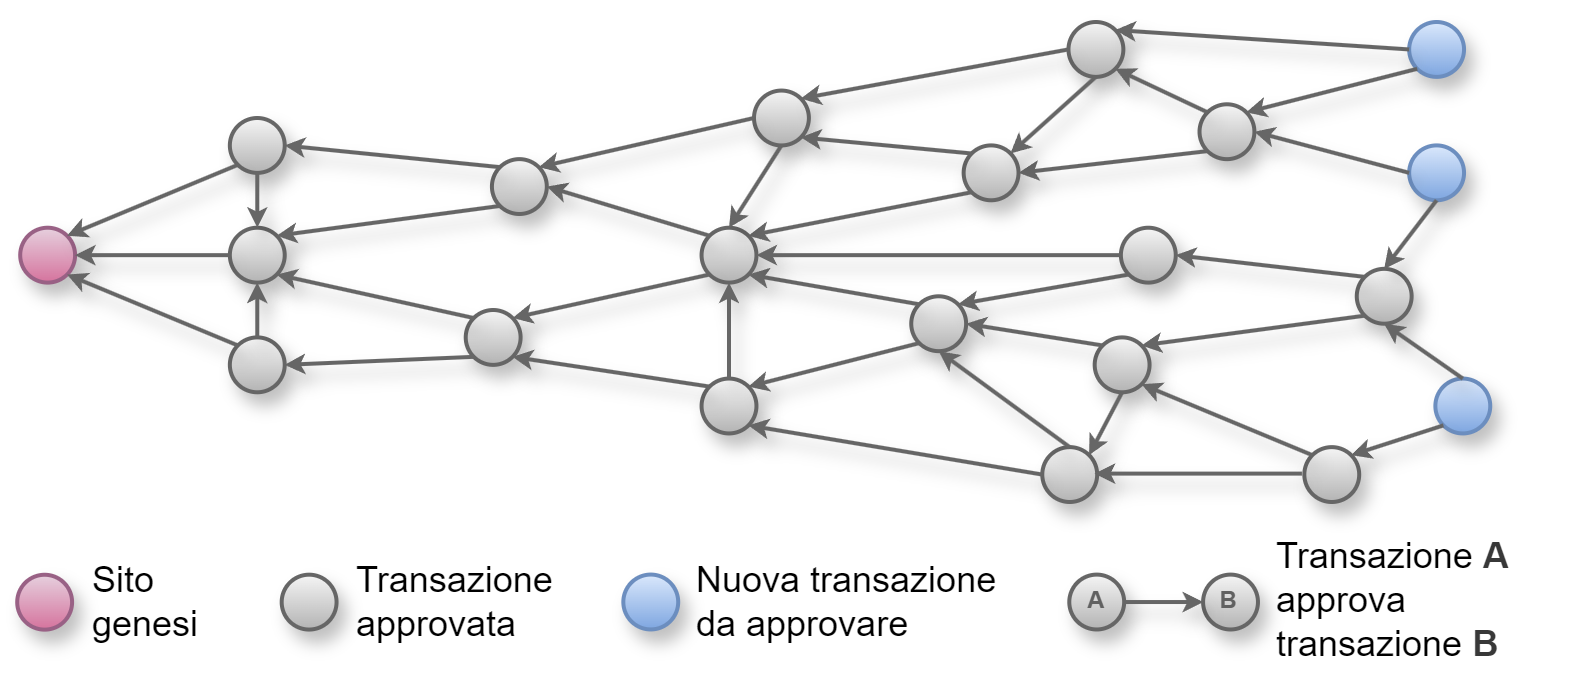
\includegraphics[width=0.9\textwidth]{figures/my_tangle.png}
\caption[Il Tangle]{Struttura DAG del Tangle}\label{fig:tangle}
\end{center}
\end{figure}
Nella struttura del Tangle, ogni nodo (da qui in poi definito \textit{sito}) corrisponde a una singola transazione effettuata, mentre gli archi che collegano i siti rappresentano le approvazioni delle transazioni. Quando viene effettuata una nuova transazione, questa viene aggiunta al grafo come sito e deve approvare due transazioni già inserite in precedenza nel Tangle. La selezione di queste due transazioni avviene tramite un apposito algoritmo di selezione (vedi \ref{selection_algorithm}). Quando due transazioni sono in conflitto\footnote{Ad esempio, nel caso di \textit{double spending}, approfondito in \ref{doublespending}.}, una delle due viene marchiata come \textit{orfana}, e da quel momento in poi le sue approvazioni indirette non verranno più considerate. Per scegliere quale transazione scartare, l'algoritmo di selezione viene rieseguito un determinato numero di volte, e si considera valida la transazione che fra le due viene scelta più volte.\\
Come si vede in Figura \ref{fig:tangle}, il grafo parte da un sito di origine, il sito \textit{genesi}. Questo viene inserito dall'indirizzo che ha originariamente coniato tutti i token della criptovaluta e che, a sua volta, li ha distribuiti tra vari indirizzi \textit{fondatori} per dare inizio al sistema di scambi\footnote{La transazione genesi, di conseguenza, è approvata indirettamente da qualsiasi transazione futura inserita nel Tangle.}. Da quel momento in poi, nessun altro token potrà più essere coniato e saranno infatti sempre gli stessi a circolare nel sistema. Questo è ciò che rende il ledger di IOTA libero da minatori di token e immune all'inflazione della moneta.

\subsection{Definizioni}
Prima di proseguire, è opportuno stabilire alcune definizioni che verranno utilizzate nella restante parte della sezione, riportate in Tabella \ref{tab:tangle_def}. 
% \begin{table}[h]
\begin{center}
\begin{longtable}{c|m{0.8\linewidth}}
\hline \hline
Nodo & Un nodo è un'entità partecipante al sistema, che effettua transazioni.\\
\hline
Sito & Un sito è una transazione effettuata, rappresentata nel Tangle.\\
\hline
Peso & Il peso di una transazione è un valore direttamente proporzionale al lavoro computazionale speso per effettuarla.\\
\hline
Peso cumulativo & Il peso cumulativo di una transazione è la somma del suo peso più il peso di tutte le transazioni che l'hanno approvata (anche indirettamente).\\
\hline
Punteggio & Il punteggio di una transazione è la somma del suo peso più il peso di tutte le transazioni che ha approvato (anche indirettamente).\\
\hline \hline
\caption[Definizioni Tangle]{Definizioni}\label{tab:tangle_def}
\end{longtable}
\end{center}
\vspace{-20mm}
\subsection{Selezione delle transazioni da approvare} \label{selection_algorithm}
È necessario capire anche \textit{come} vengono selezionate le due transazioni da approvare quando ne viene effettuata una nuova. Innanzitutto, è importante sottolineare che il sistema di IOTA non impone alcuna regola sulla scelta, bensì si basa sul concetto che per i partecipanti al sistema è più conveniente seguire lo stesso algoritmo di selezione usato dalla maggioranza.
\subsubsection{Algoritmi di selezione base}
L'algoritmo di selezione più semplice che si possa usare, e che sia anche logico, consiste semplicemente nel selezionare due \textit{tip} casualmente. Nel caso in cui siano in conflitto, la transazione da rendere orfana viene scelta quindi sempre casualmente. Una tip non è altro che una transazione che non è ancora stata approvata da nessun'altra transazione. Logicamente quindi la scelta più sensata per una transazione da approvare è sicuramente una di queste.\\
Un altro algoritmo semplice, ma un po' meno aleatorio, può essere quello di selezionare le tip che hanno un punteggio maggiore. La logica di questa scelta consiste nell'aggiungere approvazioni (e quindi anche sicurezza) al maggior numero di transazioni. Questo è perché approvare transazioni con un punteggio alto significa anche approvare indirettamente un alto numero di transazioni.
\subsubsection{Algoritmo più avanzato per prevenire attacchi double spending}
\label{doublespending}
Consideriamo ora un possibile attacco alla sicurezza del sistema, dove l'attaccante cerca di farsi approvare una doppia transazione in cui spende gli stessi token due volte (double spending). Analizziamo quindi come sia possibile migliorare la sicurezza per prevenire questi attacchi, e perché i semplici algoritmi di selezione visti in precedenza non siano sufficienti.\\
Come si vede anche in Figura \ref{fig:tangle_attack}, un attaccante potrebbe effettuare un pagamento in una transazione e, solo dopo che questa ha ricevuto un numero sufficiente di approvazioni e il venditore ha accettato il pagamento, eseguire un'altra transazione double spending. A questo punto, sfruttando la propria potenza computazionale, potrebbe inserire una serie di transazioni che approvino quella double spending (ma non quella originale), ancorandosi saltuariamente anche al Tangle principale per aumentare il proprio punteggio. In questo modo, l'attaccante riuscirebbe a creare una diramazione del Tangle (un subtangle) che parte dalla transazione double spending e si distacca da quella originale. Se riuscisse ad aggiungerci un numero sufficiente di transazioni in modo da superare l'altro subtangle, quest'ultimo verrebbe eventualmente reso orfano\footnote{Perché, seguendo algoritmi di selezione semplici come quelli descritti in precedenza, più il subtangle parassita supera quello sano, più probabilità ha che vengano selezionate le sue tip.}. In questo scenario, il ramo valido rimarrebbe quello in cui è presente la transazione double spending, consentendo all'attaccante di spendere con successo gli stessi token due volte.

\begin{figure}[h]
\begin{center}
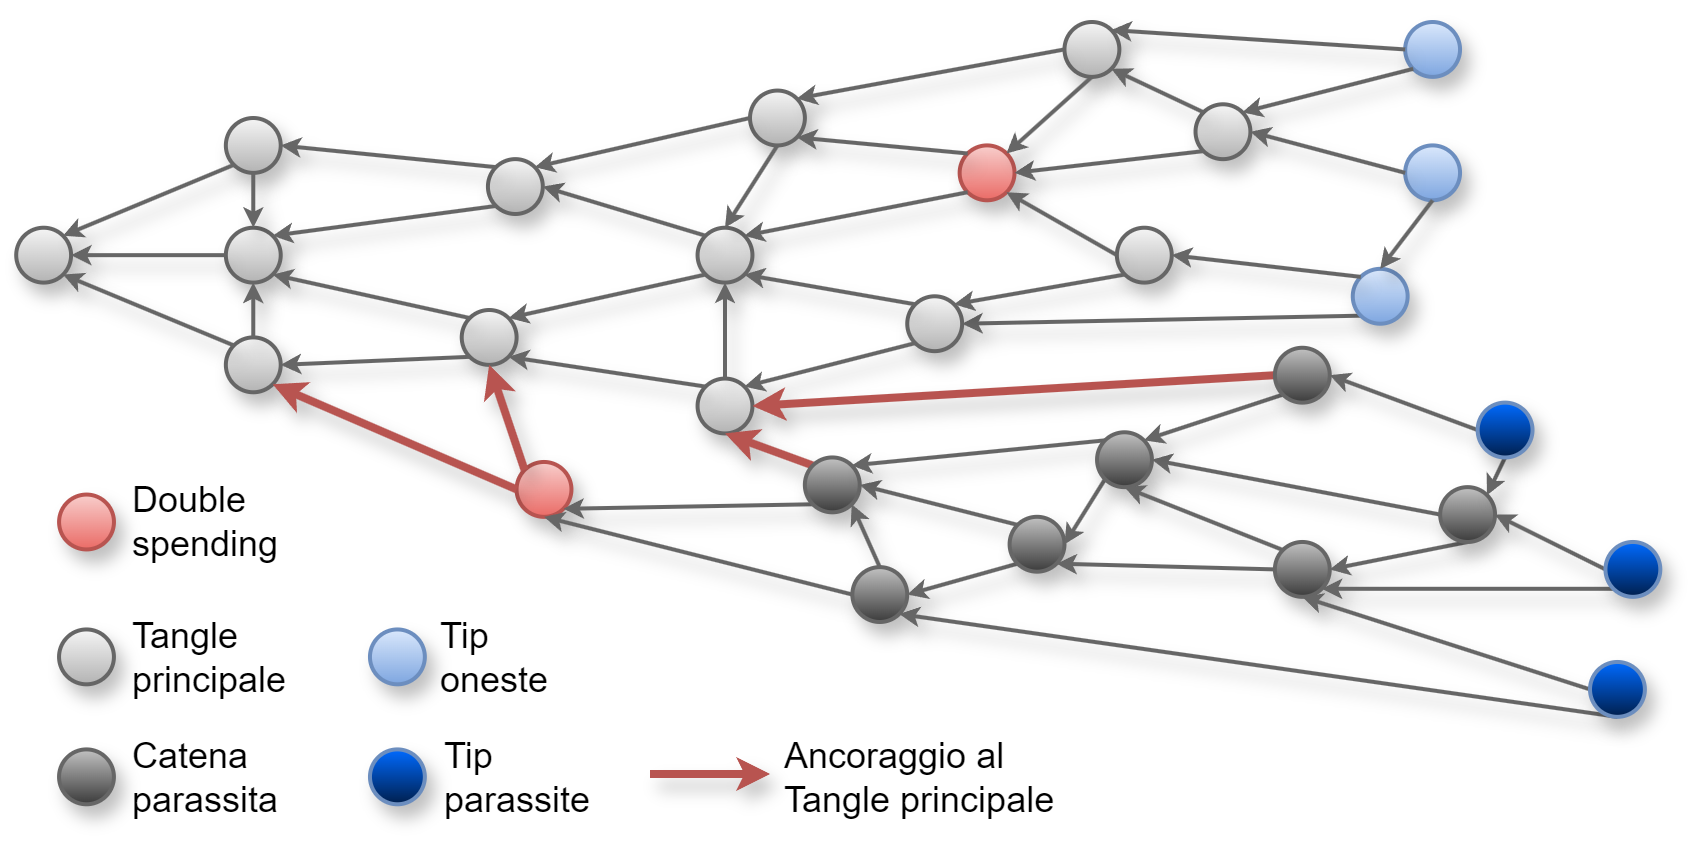
\includegraphics[width=0.9\textwidth]{figures/my_tangle_attack.png}
\caption[Attacco double spending]{Attacco double spending con un subtangle parassita}\label{fig:tangle_attack}
\end{center}
\end{figure}
Per prevenire questo tipo di attacchi, è necessario che il flusso di transazioni effettuate nel sistema sia maggiore della quantità di transazioni che la potenza computazionale dell'attaccante gli permette di eseguire. Per questo è utile (soprattutto nelle fasi iniziali del sistema, quando ancora non è molto popolato) prevedere ulteriori misure di sicurezza, ad esempio avendo dei "checkpoint" periodici in cui controllare tutte le transazioni passate. Nelle prime versioni di IOTA, questo era il compito del \textit{coordinatore}, un singolo nodo fidato che inserisce delle transazioni speciali che convalidano l'intero subtangle precedente al punto in cui si ancorano. Qualsiasi convalida effettuata dal coordinatore è irreversibile~\cite{coordinator}. In aggiornamenti successivi di IOTA, questa figura è stata sostituita da un gruppo di consenso decentralizzato (vedi \ref{coordicide}).\\
Bisogna però considerare anche la possibilità in cui l'attaccante crei \textit{in anticipo} una catena di transazioni sopra a quella double spending, per poi attaccarla al Tangle nel momento in cui la transazione originale viene approvata. In questo modo, la difesa non può più basarsi esclusivamente sulla potenza computazionale. È possibile però utilizzare un algoritmo di selezione più avanzato, in modo che non vengano approvate le transazioni di un eventuale subtangle parassita aggiunto dall'attaccante. Come illustrato in Figura \ref{fig:random_walk}, l'algoritmo consiste nel selezionare un certo numero di siti nel Tangle, e far partire da essi dei percorsi aleatori verso le tip. Questi percorsi si spostano fra i siti seguendo gli archi del Tangle. La selezione dei siti da cui partire è arbitraria, ma deve essere in un range di distanza dalle tip ragionevole: se è troppo vicino, l'algoritmo risulta poco efficace; se è troppo lontano, i tempi di calcolo diventano eccessivi. I primi due percorsi che terminano raggiungendo una tip, selezioneranno le due tip da approvare.

\begin{figure}[h]
\begin{center}
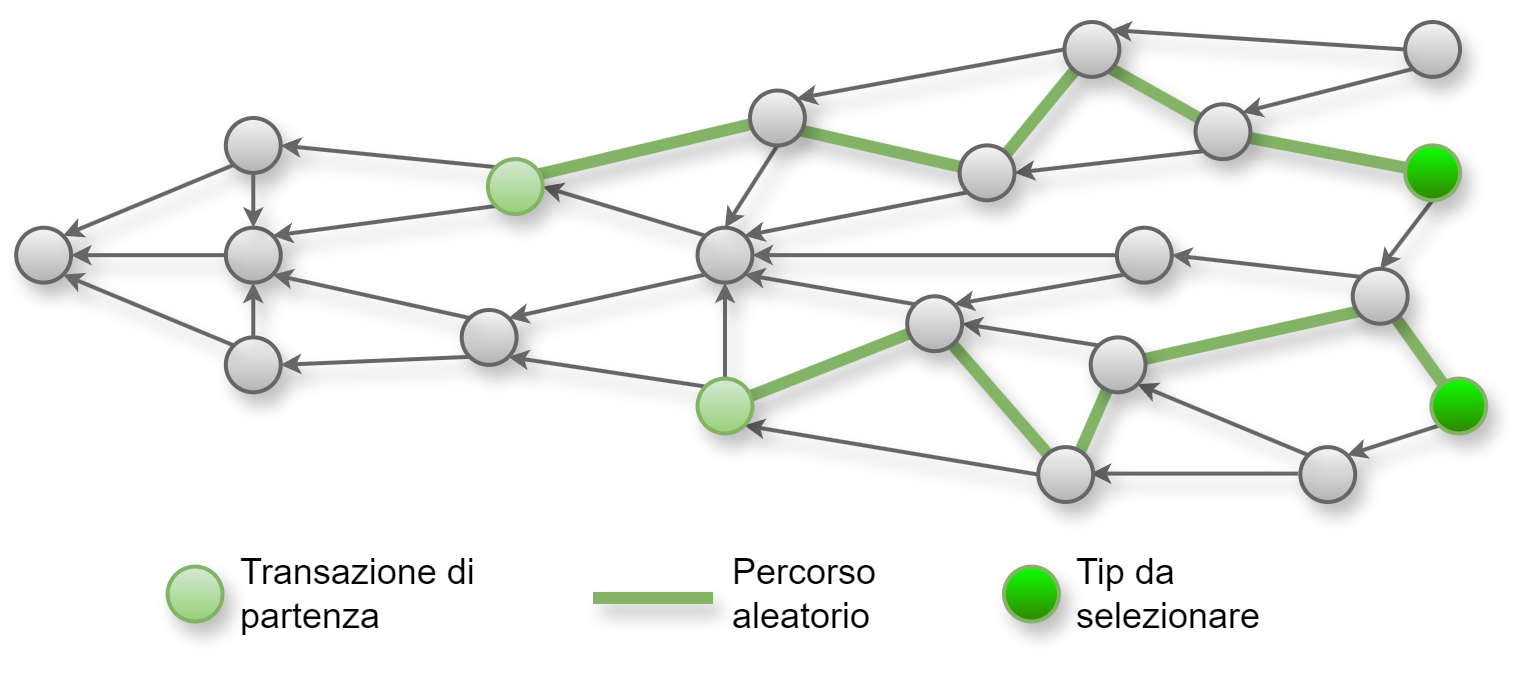
\includegraphics[width=0.9\textwidth]{figures/my_random_walk.png}
\caption[Percorsi aleatori]{Algoritmo di selezione basato su percorsi aleatori}\label{fig:random_walk}
\end{center}
\end{figure}
Per la scelta del percorso da prendere, ad ogni passo viene calcolata una distribuzione di probabilità per decidere in quale sito spostarsi. Questa distribuzione di probabilità dipende dalla differenza del peso cumulativo fra il sito attuale e quello di destinazione. Maggiore è questa differenza, minore è la probabilità che il percorso prenderà la strada verso quel sito.\\
Di conseguenza, la probabilità che il percorso aleatorio finisca all'interno della catena aggiunta dall'attaccante è molto bassa. Infatti, i siti appartenenti a quella singola catena avranno sicuramente un peso cumulativo inferiore rispetto ai siti dell'intero Tangle, generando quindi una differenza maggiore.

\section{Modello del ledger di IOTA}
\label{iotamodel}
È importante comprendere anche come vengono salvati e gestiti gli account dei nodi del sistema e i loro token. IOTA segue un modello chiamato \acrshort{utxo} ledger model. Questo modello si basa sul concetto di \acrfull{utxo}. Ogni account del ledger, associato a un indirizzo, possiede un determinato numero di \acrshort{utxo}, ognuno dei quali contiene un certo valore di token. Quando si effettua una transazione, vengono utilizzati come input un certo numero di \acrshort{utxo} del mittente, che vengono poi distrutti per produrne di nuovi da assegnare al destinatario. Da qui deriva il nome di \acrlong{utxo}: gli \acrshort{utxo} presenti nel ledger sono sempre quelli non ancora spesi in una transazione. La particolarità di questo modello è che permette scritture multiple: ciò significa che due o più transazioni possono modificare contemporaneamente lo stato del ledger\footnote{Soltanto se non prendono \acrshort{utxo} in comune come input.}. Questo meccanismo migliora notevolmente la scalabilità del sistema, ma implica anche che lo stato del ledger non sia oggettivo: in un determinato momento, due entità possono percepirlo in modi differenti.

\section{Evoluzione IOTA: Multi-ledger e Smart Contracts}
La modifica apportata a IOTA che ha maggiormente rivoluzionato il sistema, e che costituisce la base del progetto di questa tesi, è stata l'introduzione di un secondo ledger (Layer 2) sopra al classico Tangle (Layer 1)~\cite{smartcontracts}. Come illustrato anche in Figura \ref{fig:l2_structure}, questo ledger è composto da multipli ledger paralleli, basati sulla struttura classica di blockchain, che si attaccano direttamente al Layer 1. Inoltre, queste blockchain sono programmabili tramite codici immutabili che vi vengono inseriti: gli Smart Contract.

\begin{figure}[h]
\begin{center}
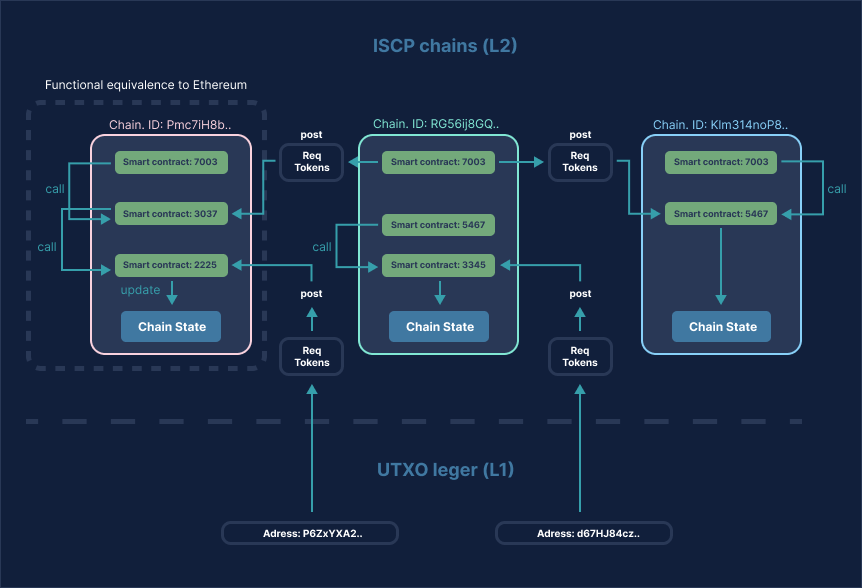
\includegraphics[width=\textwidth]{figures/l2_structure.png}
\caption[IOTA Layer 2]{Blockchain parallele nel Layer 2 ancorate su account nel Layer 1\footnotemark}\label{fig:l2_structure}
\end{center}
\end{figure}
La struttura multi-ledger introdotta permette quindi di avere un numero potenzialmente illimitato di chain programmabili, che possono eseguire in parallelo. Questo elimina uno dei principali difetti delle blockchain, ovvero la scarsa scalabilità. Allo stesso tempo, consente alle varie chain parallele di comunicare tra loro, grazie all'utilizzo del Layer 1 come canale comune.\\
L'obiettivo principale di questa struttura è fornire un metodo per programmare funzionalità anche complesse, che possano richiedere scambi di denaro. In questo modo, si favorisce l'applicazione dell'ecosistema di ledger distribuiti ad ambiti più ampi, andando oltre i semplici acquisti tramite criptovalute. Inoltre, un altro scopo è quello di consentire la tokenizzazione di qualsiasi asset, non limitandosi quindi al solo token IOTA (vedi \ref{utxo_extension}). Questo permette un ulteriore ampliamento dei possibili ambiti di utilizzo.
\footnotetext{Fonte: \url{https://archive.ph/DhqHS}}
\subsection{Struttura delle chain nel Layer 2}
Ogni blockchain che fa parte del Layer 2 ha le seguenti proprietà:
\begin{itemize}
    \item Un indirizzo proprio, chiamato chain ID, col quale si identifica la chain stessa. Tale indirizzo è immutabile.
    \item Un indirizzo sul Layer 1, al quale si ancora la chain. Tale indirizzo è separato dal chain ID, permettendo la possibilità di cambiare indirizzo proprietario della chain.
    \item Una quantità di \acrshort{utxo}, posseduti dall'account proprietario e utilizzabili dalla chain.
    \item Uno stato, che consiste in coppie chiave-valore. Lo stato è salvato in un database in tutti i nodi che hanno accesso alla chain.
    \item Multipli smart contract, che modificano lo stato.
    \item Un gruppo di validatori, nodi che mantengono la costanza dello stato nel sistema distribuito raggiungendo un consenso.
\end{itemize}
\subsection{Aggiornare lo stato di una chain}
Il meccanismo con cui una chain aggiorna il proprio stato consiste nel prendere in input degli asset (\acrshort{utxo}) che arrivano all'account della chain e, successivamente, aggiornare il proprio stato in base alle computazioni degli smart contract. Tuttavia, come già detto, lo stato degli account del ledger in L1 non è oggettivo. È quindi necessario concordare un unico stato del ledger, in modo da poter produrre uno stato oggettivo della chain.\\
È per questo motivo che ad ogni chain è assegnato un certo numero di validatori. Un validatore è un'entità, come una persona o un'azienda, che insieme ad altri validatori va a formare il comitato dei validatori della chain. Il compito di questo comitato di validatori è appunto quello di mantenere oggettivo lo stato della chain. Per raggiungere questo obiettivo, il comitato segue un algoritmo di consenso \acrfull{bft}, che gli permette di raggiungere un consenso finché ci siano almeno \(\dfrac{2}{3}N+1\) validatori non malevoli nel comitato di \(N\) validatori\footnote{Sono necessari \(\dfrac{1}{3}N\) validatori malevoli per impedire la produzione di uno stato valido, e \(\dfrac{2}{3}N+1\) per crearne uno falsificato.}.\\
Prima che la chain prenda in input degli asset per modificare il proprio stato, i validatori concordano quindi su uno stato del ledger di L1 da considerare oggettivo e sull'ordine degli input da processare. Una volta effettuate le operazioni e modificato lo stato della chain, questo viene depositato tramite una transazione come asset del chain account. La transazione è accettata soltanto se i validatori forniscono una \textit{threshold signature} valida di tale transazione, ovvero una firma ottenuta dalla somma di tutte le firme dei validatori cooperanti (che, come prima, basta siano più di due terzi dei validatori totali).\\
In questo modo, viene garantito il consenso globale sullo stato della chain, assicurandone l'unicità e l'oggettività per tutti i nodi.
\subsubsection{State anchoring}
Il processo di salvare lo stato della chain come asset del suo account su L1 viene definito state anchoring.\\
Nel dettaglio, il chain account possiede i seguenti asset:
\begin{description}[font=$\bullet$\:\:,leftmargin=\parindent,labelindent=\parindent]
  \item[Asset della chain] \acrshort{utxo} che sono collegati e controllati dalla chain tramite valori nel suo stato.
  \item[Richieste per la chain] \acrshort{utxo} in input da chi vuole utilizzare la chain, che devono ancora essere processati. Una volta processati saranno poi aggiunti agli asset della chain.
  \item[Alias output] Un \acrshort{utxo} contenente lo state anchoring della chain, che a sua volta contiene:
  \begin{itemize}[label=$\circ$]
      \item L'ID della chain
      \item L'ID del chain account
      \item Un timestamp dello state anchoring
      \item L'indice di stato, che aumenta ad ogni state anchoring
      \item Una prova crittografica del nuovo stato della chain. Viene utilizzata la radice del \textit{Verkle Tree} (una versione più efficiente del Merkle Tree, vedi \ref{verkletree}) calcolato dallo stato della chain.
  \end{itemize}
\end{description}
Ogni volta che avviene uno state anchoring, viene eliminato il precedente alias output e sostituito con quello nuovo, in modo che ci sia sempre e solo un alias output per ogni chain.\\
Grazie alla prova crittografica, viene assicurato che lo stato sia protetto da manomissioni e che sia uguale per tutti i nodi.
\subsubsection{State synchronization}
\label{state_sync}
In una sezione dello stato della chain chiamata \textit{blocklog} sono anche presenti i blocchi passati della blockchain, così da poterli utilizzare come cronologia per ricostruire lo stato. Se un nodo infatti si accorge che il suo indice di stato e la sua prova crittografica dello stato sono diversi da quelli nello state anchor, significa che non è sincronizzato con lo stato attuale. A quel punto, confrontando l'indice di stato, il nodo può determinare di quanti blocchi è indietro e richiedere ad altri nodi i blocchi necessari per ricostruire lo stato attuale partendo dal proprio. Questo processo è definito state synchronization.
\subsection{Funzionamento degli Smart Contract}
Come già introdotto prima, uno Smart Contract è un programma eseguito su chain che modifica il suo stato, producendo sempre un output deterministico e oggettivo per tutti i nodi. Il suo codice, immutabile, è salvato nello stato della chain, e ogni smart contract ha a sua disposizione una partizione dello stato per salvare i propri dati.\\
L'esecuzione dei codici avviene grazie alla \acrfull{vm}, una parte della chain composta da interpreti di codice e da smart contract predefiniti, necessari al funzionamento della chain. Tutti gli altri smart contract inseriti nella chain vengono aggiunti alla \acrshort{vm} come estensione di essa. La \acrshort{vm} di IOTA segue lo stesso modello della \acrfull{evm} di Ethereum: gli smart contract programmati per quest'ultima sono infatti compatibili anche con la \acrshort{vm} di IOTA.\\
Per garantire flessibilità, la \acrshort{vm} offre inoltre astrazioni e interfacce per le sue funzioni principali, permettendo il supporto di multipli tipi di interpreti e di smart contract, anche sulla stessa chain. Un'altra componente essenziale della \acrshort{vm} è il \textit{Sandbox}, un'interfaccia che permette agli smart contract di avere accesso alle risorse della chain. L'accesso viene regolato in modo strettamente deterministico, consentendo sempre l'esecuzione di un solo smart contract alla volta. È quindi grazie al Sandbox che viene assicurato che gli smart contract della chain producano sempre un risultato deterministico e oggettivo per tutti i nodi.

\subsubsection{Richiamare uno Smart Contract}
Esistono due modi in cui le funzioni di uno smart contract possono essere richiamate:
\begin{enumerate}
    \item Tramite semplici chiamate sincrone effettuate da altri smart contract all'interno della stessa chain.
    \item Tramite chiamate dall'esterno della chain che prendono il nome di \textit{richieste}. Sono quelle che vanno a formare gli asset in input della chain.
\end{enumerate}
Le richieste possono a loro volta essere effettuate in due modi: on-ledger e off-ledger.
\begin{description}[font=$\bullet$\:\:,leftmargin=\parindent,labelindent=\parindent]
  \item[Richieste on-ledger] Richieste effettuate tramite transazioni su L1, con il chain ID come destinatario. Sono utilizzate quando il richiedente è un indirizzo del ledger e la chiamata prevede lo scambio di asset L1, oppure quando il richiedente è uno smart contract di un'altra chain.
  \item[Richieste off-ledger] Richieste invece effettuate senza passare per il ledger di IOTA, tramite chiamate API a uno degli \textit{access nodes}\footnote{I nodi, fra i quali i validatori, che hanno accesso alla chain e possiedono il database con il suo stato.} della chain. Queste richieste sono molto più veloci ed efficienti e vengono utilizzate se il richiedente è un indirizzo che non ha necessità di scambiare asset L1 tramite la chiamata\footnote{E quindi, non ha necessità di utilizzare il ledger.}. In questo caso, la richiesta viene propagata al backlog della chain tramite un meccanismo di disseminazione tra gli access nodes.
\end{description}

\subsubsection{Considerazioni sulle tasse}
Nonostante il ledger di IOTA sia libero da tasse, è comunque necessario imporre in L2 dei limiti nell'utilizzo degli smart contract per prevenire abusi da parte dei richiedenti. Per questo motivo viene introdotto il concetto di \textit{gas}. Ogni utilizzo delle risorse della chain richiede un certo quantitativo di gas, direttamente proporzionale alla quantità di risorse utilizzate. Quando viene invocata una funzione di uno smart contract che modifica lo stato della chain, viene quindi consumato il quantitativo di gas necessario. Al contrario, se viene invocata una funzione che non effettua alcuna modifica allo stato (chiamate funzioni \textit{view}) non viene consumato nessun gas.\\
Il modo per ottenere gas e i limiti sul suo utilizzo sono stabiliti da chi gestisce la chain. La politica più utilizzata prevede una tassa sul consumo di gas, convertendo gli IOTA in gas. In questo scenario, le tasse pagate alla chain vengono suddivise fra i validatori e il proprietario della chain. Sono comunque possibili anche altri tipi di politiche sul gas, come ad esempio non imporre alcun limite, oppure rendere l'acquisizione di gas libera da tasse ma imporre un limite massimo prefissato sul suo consumo.

\subsubsection{Smart Contract predefiniti}
Come detto in precedenza, la \acrshort{vm} di IOTA è fornita di base con un certo numero di smart contract (definiti \textit{core smart contracts}) necessari al funzionamento della chain, elencati qui di seguito in Tabella \ref{tab:core_contracts}.
\newpage
\begin{center}
\begin{longtable}{c|m{0.8\linewidth}}
\hline \hline
Root & Lo smart contract radice è necessario per effettuare il deploy di nuovi smart contract e per mantenere il registro di quelli esistenti.\\
\hline
Accounts & Lo smart contract degli account permette la registrazione di account sulla chain stessa. A differenza di L1, viene adottato il modello classico delle blockchain, ovvero il modello basato su account (Vedi \ref{accountmodel}). Ogni account è identificato da un account ID, che corrisponde all'account L1 del proprietario. Questo permette agli utenti di spostare qualsiasi proprio asset da L1 alla chain. L'Accounts Contract, oltre a mantenere il registro degli account, si occupa anche di gestire lo scambio di asset fra di essi.\\
\hline
Blob & Lo smart contract dei \acrfull{blob} mantiene il registro dei dati di grandi dimensioni.\\
\hline
Blocklog & Lo smart contract del log dei blocchi è quello che mantiene la traccia e la cronologia dei blocchi nella chain (Come visto in \ref{state_sync}).\\
\hline
Governance & Lo smart contract della governance si occupa di gestire gli aspetti amministrativi della chain. Alcuni esempi sono la gestione dei diritti di accesso, delle politiche riguardanti tasse e gas, o della sostituzione dei validatori.\\
\hline
$\textunderscore$default & Uno smart contract di default che viene chiamato automaticamente quando arriva una richiesta a uno smart contract non esistente.\\
\hline \hline
\caption[Core Smart Contracts]{I core smart contract della \acrshort{vm} di IOTA}\label{tab:core_contracts}
\end{longtable}
\end{center}

\subsection{Estensione dell'\acrshort{utxo} ledger model}
\label{utxo_extension}
L'\acrshort{utxo} ledger model di base permette soltanto di avere \acrshort{utxo} contenenti valori del token nativo (in questo caso, IOTA). Per poter permettere l'implementazione del Layer 2 e delle sue multi-chain, è stato quindi necessario per IOTA aggiungere un'estensione al modello che introduca tipi di \acrshort{utxo} speciali. Inoltre, l'estensione aggiunge anche la possibilità di destinare \acrshort{utxo} all'indirizzo di una chain. Normalmente ciò non sarebbe possibile perché, per permettere il cambio di proprietario, l'indirizzo della chain non è vincolato all'indirizzo del nodo su cui è ancorata.\\
I tipi di \acrshort{utxo} aggiunti con questa estensione sono i seguenti:

\begin{description}[font=$\bullet$\:\:,leftmargin=\parindent,labelindent=\parindent]
  \item[Alias output] Permette lo state anchoring e la creazione degli alias output delle chain. Come detto in precedenza, è presente anche un vincolo che impone uno e un solo alias output per ogni chain.
  \item[Foundry output] Rende possibile la tokenizzazione avanzata, ovvero la creazione di asset diversi dal token IOTA (chiamati \textit{asset nativi}). In questo modo, diventa possibile la tokenizzazione di qualsiasi cosa. Può esistere un solo foundry output per ogni tipo di token creato. Tale foundry output contiene il bilancio del token e permette al suo gestore di coniarne o distruggerne qualsiasi quantità\footnote{Al contrario del token IOTA, che non è né coniabile né distruggibile dopo la creazione del sistema.}.
  \item[\acrshort{nft} output] Permette l'utilizzo di \acrfull{nft} come asset nativi. È consentito un unico \acrshort{nft} output per uno specifico ID. Un \acrshort{nft} output inoltre contiene una prova di origine immutabile, ovvero la chiave pubblica di chi lo ha creato.
  \item[Extended value transfer output] Quello che effettivamente permette lo scambio anche di asset nativi, estendendo i normali \acrshort{utxo} e fornendo vincoli aggiuntivi. È sempre tramite questo output inoltre che vengono inviate le richieste alle funzioni degli smart contract sulle chain.
\end{description}

\section{IOTA 2.0: Mana e economia sostenibile}
L'aggiornamento 2.0 di IOTA, uno dei più recenti, rappresenta un'altra evoluzione importante in quanto introduce due novità di svolta:
\begin{enumerate}
    \item Un nuovo metodo di consenso decentralizzato, che sostituisce il ruolo del coordinatore nel validare lo stato del Layer 1.
    \item Una risorsa chiamata \textit{Mana}, che rivoluziona il modo in cui vengono forniti incentivi ai nodi partecipanti al ledger~\cite{iota20}.
\end{enumerate} 
Il Mana è una risorsa che viene generata da un nodo in due possibili modi:
\begin{enumerate}
    \item Mantenendo nel proprio wallet dei token IOTA. Viene generato Mana passivamente finché ci sono IOTA nel proprio account. Più IOTA si possiedono, maggiore è la quantità di Mana generata. È importante tener conto anche che alla quantità di Mana generata nel tempo è applicata una funzione di decadimento, che riduce progressivamente la quantità di Mana ottenuto. Questa funzione è stata introdotta per disincentivare l'accumulo eccessivo di token senza una reale partecipazione alla rete, evitando che gli utenti trattengano IOTA al solo scopo di generare Mana.
    \item Partecipando attivamente alla sicurezza della rete, agendo come validatore o delegatore  (Vedi \ref{coordicide}).
\end{enumerate}
Allo stesso tempo, il Mana è anche la risorsa necessaria per poter utilizzare la rete ed effettuare transazioni. In questo modo, gli incentivi per partecipare alla rete sono puramente pratici e ne beneficeranno quindi soltanto coloro che sono genuinamente interessati a partecipare e contribuire al sistema.\\
Tutte le azioni necessarie ad accumulare Mana (e quindi, a poter utilizzare la rete) prevedono un acquisto di token IOTA\footnote{Ma non necessariamente una spesa, concetto fondamentale che differenzia IOTA dagli altri token (Vedi \ref{manaconsensus}).}. Questo comporta contemporaneamente due vantaggi:
\begin{enumerate}
    \item Incentivando ad acquistare token IOTA, il token aumenta di valore.
    \item Imponendo la necessità di possedere token per utilizzare la rete, aumenta la protezione dagli attacchi di Sybil\footnote{Attacchi in cui una singola entità malevola può utilizzare multipli nodi per partecipare alla rete, e utilizzarne l'ampio numero per compiere azioni a suo vantaggio.}.
\end{enumerate}
Grazie al Mana inoltre, unito alla politica senza tasse di IOTA, si va a creare un'economia ancora più bilanciata. Tale economia infatti, evita il fenomeno in cui si arricchiscono sempre di più i validatori a scapito degli altri partecipanti tramite tasse e premi in token per i loro servizi. Si ricorre invece a un sistema in cui i premi per chi fa da validatore consistono in Mana, senza alterare il bilancio dei token di nessuna entità. In questo modo, chi aiuta a validare la rete riceve comunque dei compensi, ma senza creare uno squilibrio crescente nella distribuzione dei token.
\subsection{Staking e sistema di consenso}
\label{coordicide}
Con IOTA 2.0, il ruolo di un unico coordinatore centrale è stato sostituito da un metodo di consenso decentralizzato, in cui chiunque può partecipare alla validazione delle transazioni agendo come validatore o delegatore. Per farlo è necessario fare lo \textit{staking} di una parte dei propri token IOTA, ovvero "congelarli" nel caso dei validatori o scommetterli su un validatore nel caso dei delegatori.
\subsubsection{Validatori}
Per diventare validatore è necessario prima iscriversi a una lista di possibili validatori. Per farlo, un nodo deve inserire uno speciale \acrshort{utxo} contenente le informazioni necessarie, chiamato \textit{staking feature}, nello stato del proprio account. È necessario inoltre fare lo staking di una parte dei propri token IOTA, che rimarranno congelati fintanto che si è iscritti.\\
Dalla lista dei possibili validatori vengono poi selezionati quelli effettivi, che opereranno per un determinato periodo di tempo chiamato \textit{epoca}, e saranno sostituiti a ogni nuova epoca. Il parametro principale utilizzato nella scelta è il \textit{peso} del validatore, dato dalla quantità di token con cui ha fatto lo staking sommata alla quantità di token che gli sono stati delegati da altri nodi. È inoltre da considerare che i token delegati hanno un valore inferiore rispetto a quelli messi direttamente in staking dal validatore. Questo sistema evita che un validatore abusi della delegazione, delegando token a sé stesso per ottenere lo stesso peso dello staking ma senza congelare i propri fondi.\\
Il compito di un validatore è inserire \textit{transazioni di validazione} per raggiungere il consenso sullo stato del ledger con gli altri validatori. Con ogni transazione di validazione si esprime il proprio voto su tutto il sub-tangle a cui viene ancorata.\\
Le transazioni di validazione sono leggere, contengono solo i dati essenziali, hanno priorità maggiore e non costano Mana. Questo garantisce di poterle sempre inserire adeguatamente nel ledger senza però congestionare la rete per le altre transazioni.\\
Alla fine di un'epoca, un validatore viene ricompensato se ha raggiunto la quota minima richiesta di transazioni di validazione inserite. La quantità di Mana ottenuta dal validatore dipende dal numero totale di transazioni di validazione che ha effettuato, da quanto queste hanno aiutato a raggiungere il consenso e dal peso del validatore.
\subsubsection{Delegatori}
Se dei nodi non vogliono fare da validatori ma desiderano comunque ottenere del Mana senza dover congelare i propri token, possono delegarli a uno dei validatori. Per delegare dei token è necessario inserire nel proprio account uno speciale \acrshort{utxo}, chiamato \textit{delegation output}, che contiene la quantità di token delegati e l'indirizzo del validatore a cui si intende delegarli. Come detto in precedenza, questa operazione non congela i propri token, al contrario dei validatori. Di conseguenza, un delegatore è libero di spenderli anche dopo averli delegati, oppure anche di ri-delegarli a un altro validatore.\\
È inoltre importante specificare che è possibile delegare anche token presenti sulle chain di L2, poiché anche una chain stessa può delegare il proprio potere a un validatore per ottenere Mana.
\subsubsection{Distribuzione delle ricompense in Mana}
Al termine di un'epoca, le ricompense vengono distribuite tra validatori e delegatori secondo una proporzione 1:2:3. Questo significa che, se il Mana generato passivamente dal possesso di \(x\) token è \(1x\), quello ottenuto delegando la stessa quantità di token è \(2x\), mentre quello ottenuto facendone lo staking come validatore è \(3x\). Le ricompense sono adeguate in quanto aumentano proporzionalmente alla "posta in gioco" messa e al contributo fornito.

\section{Differenze con altri ledger}
Confrontiamo ora più direttamente IOTA con altre strutture di blockchain, rivedendone i concetti chiave. Ci sono molti fattori a differenziare IOTA dagli altri ledger esistenti, e che lo portano ad essere un passo importante verso l'evoluzione dei sistemi di transazioni digitali e criptovalute.
\subsection{Layer 1}
La differenza principale, come visto all'inizio di questo capitolo, consiste nella struttura stessa del ledger che si distacca dalla classica struttura di blockchain nel suo Layer 1. Come infatti illustrato in Figura \ref{fig:blockchain_bottleneck}, con la sua struttura a \acrshort{dag}, IOTA sostituisce il problema principale di scalabilità delle classiche blockchain, che sono invece limitate a poter aggiungere un solo blocco alla volta alla chain\footnote{\url{https://archive.is/cZqhQ}}. 

\begin{figure}[h]
\begin{center}
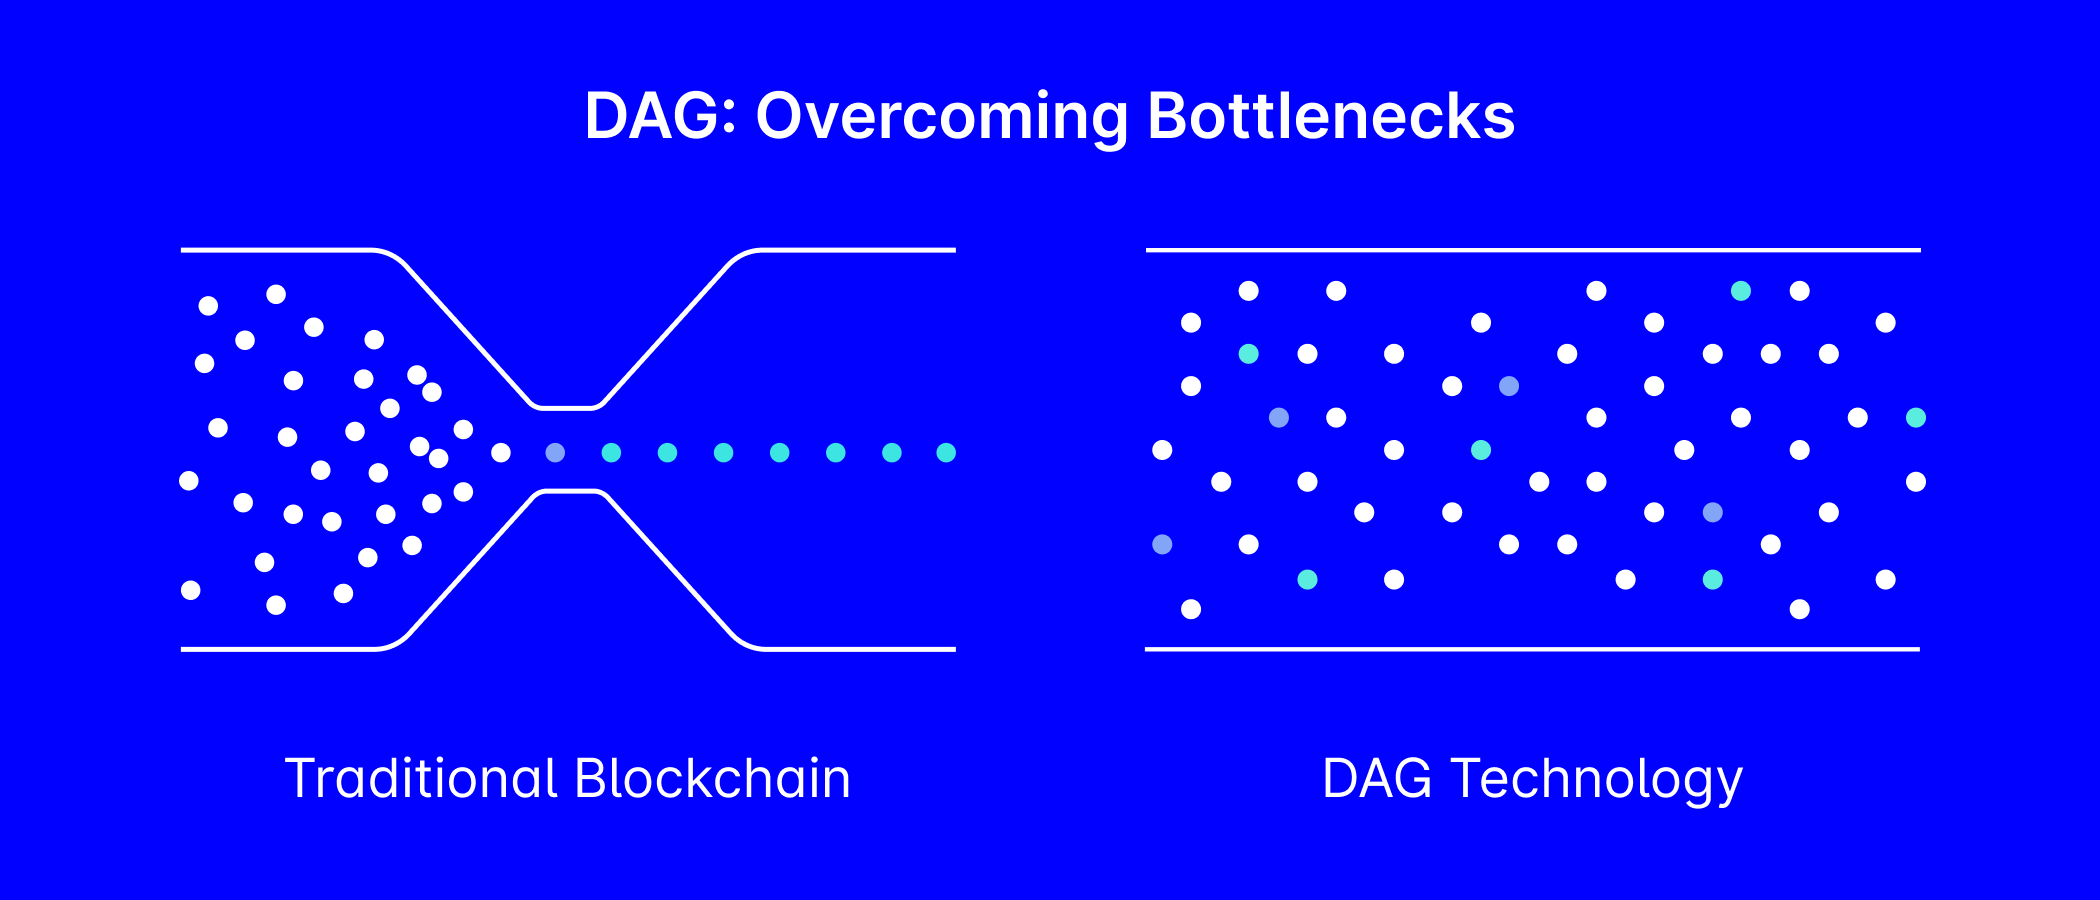
\includegraphics[width=\textwidth]{figures/blockchain_bottleneck.png}
\caption[Blockchain bottleneck]{La scalabilità del \acrshort{dag} risolve il bottleneck delle \linebreak classiche blockchain\footnotemark}\label{fig:blockchain_bottleneck}
\end{center}
\end{figure}
\label{accountmodel}
Come già visto però, rimuovendo il limite di inserimento di una transazione alla volta il \acrshort{dag} porta anche a uno stato del ledger non oggettivo, che in un determinato momento può non essere visto allo stesso modo da due nodi diversi. Questo ha reso naturale l'adozione dell'\acrshort{utxo} ledger model (vedi \ref{iotamodel}), al contrario di altri ledger basati su blockchain, che spesso (ma non sempre\footnote{Bitcoin, anche se ha la struttura di una blockchain classica, utilizza \acrshort{utxo} ledger model. Ethereum invece utilizza il modello basato su account.}) si affidano al modello basato su account. Questo modello, al contrario dell'\acrshort{utxo} ledger model che non ha uno stato oggettivo, è formato da account che sono entità atomiche con dei bilanci. Queste possono essere aggiornate soltanto una per volta, rendendo lo stato del ledger oggettivo~\cite{smartcontracts}.\\
Il metodo delle blockchain tradizionali di aggiungere un blocco alla volta introduce anche un'altra caratteristica tipica in cui IOTA si differenzia: il metodo di inserimento dei blocchi. Tipicamente infatti, nella rete di una blockchain sono presenti delle autorità centrali a cui bisogna rivolgersi per potersi far aggiungere le transazioni nei blocchi da inserire nella chain. In IOTA invece, ogni nodo ha la possibilità di inserire manualmente le proprie transazioni in qualsiasi momento.\\
\footnotetext{Fonte: \url{https://archive.is/cZqhQ}}
Un'altra differenza importante, su cui IOTA basa la sua politica, è l'assenza di tasse e di mining di token. IOTA infatti si impegna a non imporre alcuna tassa per la creazione di transazioni, come invece accade tipicamente nei ledger distribuiti. Ne permette invece la creazione liberamente senza costi aggiuntivi, implementando poi con IOTA 2.0 uno strumento per rafforzare questo metodo: l'utilizzo di Mana per creare transazioni, ottenibile semplicemente partecipando alla rete. Come detto, in IOTA è inoltre assente anche il concetto di mining di nuovi token, in quanto tutti i token IOTA in circolazione vengono creati in un'unica volta alla creazione della rete, dopo la quale non è più possibile coniarne o distruggerne. Questo evita l'altrimenti inevitabile fenomeno di inflazione dei token, comune nelle blockchain in cui i nodi effettuano regolarmente mining per coniare nuovi token.\\
Con IOTA 2.0 e l'introduzione di un comitato di consenso, emergono ulteriori differenze influenti rispetto alla gestione delle autorità di validazione negli altri ledger.

\begin{figure}[h]
\begin{center}
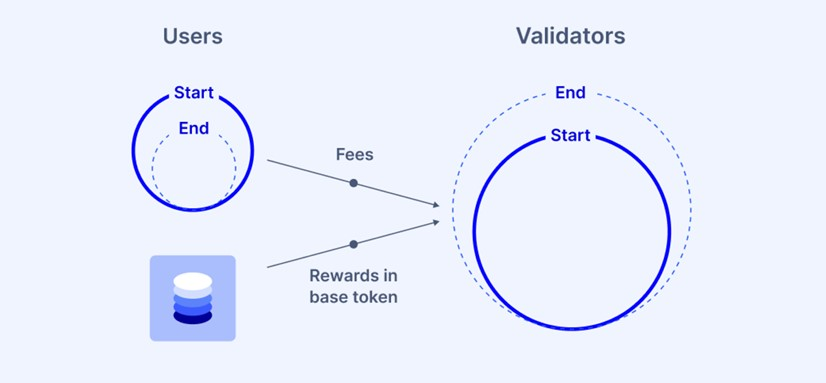
\includegraphics[width=\textwidth]{figures/ledger_economy.jpg}
\caption[Arricchimento dei validatori]{Come tasse e ricompense in token influiscono sullo sbilanciamento dell'economia nella blockchain\footnotemark}\label{fig:ledger_economy}
\end{center}
\end{figure}
\footnotetext{Fonte: \cite{iota20}}
\label{manaconsensus}
Come infatti viene illustrato in Figura \ref{fig:ledger_economy}, solitamente in una blockchain i nodi di validazione vengono costantemente premiati tramite token, sia con le tasse pagate dai nodi partecipanti sia con le ricompense ottenute tramite validazione della rete. Questo porta naturalmente a uno sbilanciamento sempre crescente dell'economia. È inevitabile infatti l'accumulo della ricchezza nelle mani di pochi, rendendo invece sempre più a corto la maggior parte dei normali utilizzatori della rete. IOTA invece propone un sistema, quello del Mana, che offre comunque meritati vantaggi alle autorità di validazione, ma senza basarsi su trasferimenti della valuta del ledger. In questo modo, l'economia rimane bilanciata e sostenibile per tutti.

\subsection{Layer 2}
Le chain del Layer 2, che hanno invece la classica struttura di una blockchain in cui viene inserito un blocco alla volta, adottano come modello del ledger il modello basato su account, come Ethereum.\\
Sempre come Ethereum, una chain L2 di IOTA ha il vantaggio di poter accedere direttamente all'intero stato della chain. Questo perché lo stato delle blockchain in L2 non contiene soltanto le transizioni per ricostruirlo, ma memorizza direttamente tutti i dati chiave-valore dello stato. Questo non è il caso ad esempio di Bitcoin, in cui per ottenere e ricostruire lo stato è necessario risalire i blocchi della blockchain applicando le transizioni~\cite{bitcoinethereum}. 
\label{verkletree}Inoltre, IOTA utilizza anche un metodo differente per memorizzare l'hash dello stato. Mentre in blockchain come Bitcoin o Ethereum in un blocco viene salvato il \textit{Merkle Tree}\footnote{Un albero di hash per memorizzare dati multipli. Si parte dall'hash dei dati singoli, che formano le foglie dell'albero, e si esegue l'hash delle loro somme a coppia di due (o più, nel caso di Ethereum sono 16) costruendo così l'albero, fino a raggiungere un unico hash radice~\cite{merkletree}.} dello stato, le chain L2 di IOTA utilizzano una versione più efficiente chiamata Verkle Tree. Tale versione utilizza un diverso schema crittografico rispetto alla funzione di hash del Merkle Tree, chiamato Vector Commitment, che permette di occupare meno spazio.\\
Un'altra sostanziale differenza delle chain in L2 riguarda il funzionamento della validazione. IOTA infatti si differenzia da altre blockchain, come Bitcoin ed Ethereum, adottando un metodo di validazione basato sul consenso piuttosto che sulle \acrlong{pow}. Le differenze principali riguardano questi due aspetti:
\begin{enumerate}[font=\bfseries]
    \item \textbf{Selezione dei validatori.} In un sistema di validazione basato su \acrlong{pow}, chiunque può partecipare alla validazione della blockchain, a patto di disporre di sufficiente potenza computazionale. In IOTA invece, viene effettuata un'effettiva selezione\footnote{È comunque possibile, se dovesse essercene bisogno, implementare in una chain un sistema di validazione in cui chiunque è libero di partecipare.}, tramite la quale verrà scelto un ristretto gruppo di nodi che agiranno da validatori\footnote{Come visto in precedenza, il comitato di validazione.}. In questo modo, sebbene la possibilità per gli utenti di partecipare alla validazione sia limitata dalla necessità di essere selezionati, questa selezione garantisce validatori fidati e quindi una maggiore sicurezza.
    \item \textbf{Metodo di validazione.} In un sistema di validazione basato su \acrlong{pow}, il validatore\footnote{Indicato più comunemente come minatore nel sistema \acrshort{pow}.} si occupa direttamente della creazione del nuovo blocco. La metrica su cui si basa la selezione del blocco da aggiungere è la potenza computazionale impiegata dal validatore per crearlo. Nel sistema basato sul consenso implementato da IOTA invece, il contenuto del blocco è deciso in automatico dalla \acrshort{vm}, e i validatori si limitano a esprimere il proprio voto su di esso e sui dati che la \acrshort{vm} deve prendere in input per crearlo. La scelta del blocco da aggiungere è quindi basata sulla collaborazione dei validatori e sul consenso che raggiungono. 
\end{enumerate}
I vantaggi apportati da questo diverso metodo influiscono positivamente sulla sicurezza (e sulla sua scalabilità) del sistema. Per manomettere un sistema basato su \acrlong{pow} è infatti sufficiente accumulare, anche singolarmente, una potenza computazionale che superi quella degli altri validatori. Per questo motivo, con la crescita di un sistema del genere e l'aumento della probabilità di attacchi, si cerca di avere sempre più validatori per aumentare la sicurezza della rete. Tuttavia, a lungo andare, questo causa problemi di scalabilità. In IOTA invece, oltre alla maggiore sicurezza garantita dalla necessità di essere selezionati e verificati per diventare validatori, manomettere la validazione è molto più complesso e richiederebbe un accordo fra molte entità. Come già detto in precedenza sarebbe infatti necessario che più di \(\frac{2}{3}\) di validatori si mettano d'accordo per falsificare la firma di validazione\footnote{O \(\dfrac{1}{3}\) che si mettano d'accordo per impedire la produzione di una firma valida.}. Questa cosa, in un contesto in cui solitamente i validatori non si conoscono o possono addirittura essere in competizione fra di loro, è molto poco probabile. È poco probabile allo stesso modo anche in un contesto in cui i validatori sono in collaborazione e si fidano reciprocamente, per la natura stessa di fiducia di questo rapporto.\\
Grazie a questo diverso meccanismo di validazione inoltre, IOTA previene anche un fenomeno comune nelle altre blockchain, chiamato \acrfull{mev}. Questo fenomeno si verifica quando un validatore di un sistema basato su \acrlong{pow} (minatore) analizza il flusso di transazioni in arrivo. Successivamente, poiché è lui stesso a creare il blocco, inserisce transazioni proprie che gli garantiscono un vantaggio economico in base a ciò che ha analizzato. Questo non è chiaramente possibile nelle chain L2 di IOTA, poiché appunto un validatore esprime soltanto il proprio voto sul blocco, che viene prodotto automaticamente dalla \acrlong{vm}.

\section{Una nuova strada: IOTA Rebased}
Durante la stesura di questa tesi, IOTA Foundation ha annunciato un nuovo approccio al loro sistema di ledger, che ne rivoluzionerà nuovamente il funzionamento. A novembre 2024, infatti, è stata pubblicata una proposta contenente modifiche importanti al ledger. Questa proposta è stata poi sottoposta a una votazione da parte della community ed è stata infine approvata a dicembre 2024~\cite{iotarebasedtech}. L'obiettivo principale è quello di integrare gli smart contract direttamente dentro al Layer 1.\\ 
L'approccio pensato per sviluppare IOTA Rebased è quello di includere direttamente in L1 MoveVM, una \acrlong{vm} che permette di passare dall'\acrshort{utxo} ledger model che ha sempre avuto IOTA a un modello object-oriented. In questo modo, viene reso possibile il funzionamento di smart contract anche complessi all'interno del Layer 1 stesso, senza dover necessitare del Layer 2.\\
Inoltre, IOTA Rebased prevede dei cambiamenti alle politiche principali di IOTA, ovvero quelle che prevedevano un sistema libero da tasse e senza coniazione di nuovi token. Viene infatti rimosso l'utilizzo di Mana, e le ricompense per validatori e delegatori vengono distribuite direttamente in token IOTA. I token per le ricompense verranno coniati ad ogni epoca, in una quantità costante, così da influire sempre meno sull'inflazione all'aumentare del numero totale di token. Per ridurre ulteriormente il rischio di inflazione e data anche l'eliminazione del Mana, le transazioni richiederanno una piccola tassa, il cui pagamento verrà bruciato. Tuttavia, la presenza di tasse è bilanciata da ricompense per lo staking significativamente più alte, che garantirebbero guadagni superiori rispetto alla piccola quantità spesa in tasse.\\
Dopo l'approvazione da parte della community a dicembre, una testnet è già stata pubblicata e gli sviluppi per portare IOTA Rebased al completamento sono iniziati a tutti gli effetti.
\subsection{Programmi futuri}
IOTA Rebased è un progetto ancora agli albori, che promette varie aggiunte future migliorative. La più ambiziosa è sicuramente la volontà di introdurre multiple \acrshort{vm} all'interno del ledger, affiancate alla principale MoveVM. In questo modo verrebbe fornito un elevato grado di universalità nel supporto agli smart contract scritti in diversi linguaggi. La \acrlong{vm} più ambita da portare è sicuramente la \acrshort{evm} utilizzata nel Layer 2. La sua integrazione permetterebbe definitivamente di includere in L1 anche tutti gli smart contract attualmente utilizzati in L2, creando un unico layer. Fino ad allora, il Layer 2 continuerà ad esistere e ad essere supportato~\cite{iotarebased}.

\clearpage{\pagestyle{empty}\cleardoublepage}



%%%%%%%%%%%%%%%%%%%%%%%%%%%%%%%%%%%%%%%%
% ANALISI PROGETTUALE
\chapter{Analisi progettuale}
\label{chap:projectanalysis}
% Cosa vogliamo raggiungere, perch\'e e quali sono state le vostre scelte per lo sviluppo ``su carta".
Questa tesi affronta lo sviluppo di uno Smart Contract IOTA, con lo scopo di analizzare vantaggi e complessità portati dallo sviluppo di applicazioni su piattaforme decentralizzate. In particolare, lo sviluppo sul ledger di IOTA metterà in risalto le prestazioni del multi-ledger introdotto dalla IOTA Foundation. Viene inoltre sviluppata anche un'applicazione esterna che si interfaccia con lo smart contract, in modo da analizzare anche i possibili utilizzi reali di questi programmi e come possono essere resi disponibili e utilizzati dagli utenti finali. \\
Questo capitolo illustra le scelte di progettazione per lo sviluppo dello smart contract e della sua applicazione esterna.

\section{Analisi delle funzionalità globali}
Lo smart contract che si è deciso di sviluppare deve permettere la creazione e la gestione di un sistema di lotteria. Un'entità, che corrisponde al creatore della lotteria, svolge il ruolo di gestore della lotteria. Creare una lotteria equivale ad effettuare il deploy di un'istanza dello smart contract. Al momento della creazione della lotteria, il gestore decide quanti e quali biglietti rendere disponibili e seleziona il biglietto vincente. Dopo la creazione può poi effettuare le seguenti operazioni di amministrazione e monitoraggio:
\begin{itemize}
    \item Aggiungere un nuovo biglietto ai disponibili
    \item Modificare il biglietto vincente
    \item Monitorare lo stato dei biglietti, potendo visualizzare quanti e quali sono stati venduti
    \item Terminare la lotteria per porre fine all'acquisto di biglietti
\end{itemize}
Una volta terminata la lotteria, al gestore spettano dei guadagni in token IOTA. Questi corrispondono al 30\% dei ricavi totali dalla vendita dei biglietti e possono essere liberamente ritirati dal gestore in qualsiasi momento.\\
Qualsiasi altro utente avrà invece il ruolo di partecipante alla lotteria, potendo acquistare un biglietto a un prezzo fisso di 10 IOTA. Una volta terminata la lotteria, il partecipante ha modo di visualizzare se il biglietto da lui acquistato è quello vincente. In caso positivo, può ritirare la sua vincita in token IOTA, equivalente al 70\% dei ricavi totali dalla vendita dei biglietti.\\
In Figura \ref{fig:app_diagram} è riportato lo schema principale che illustra gli scambi di denaro della lotteria. 

\begin{figure}[h]
\begin{center}
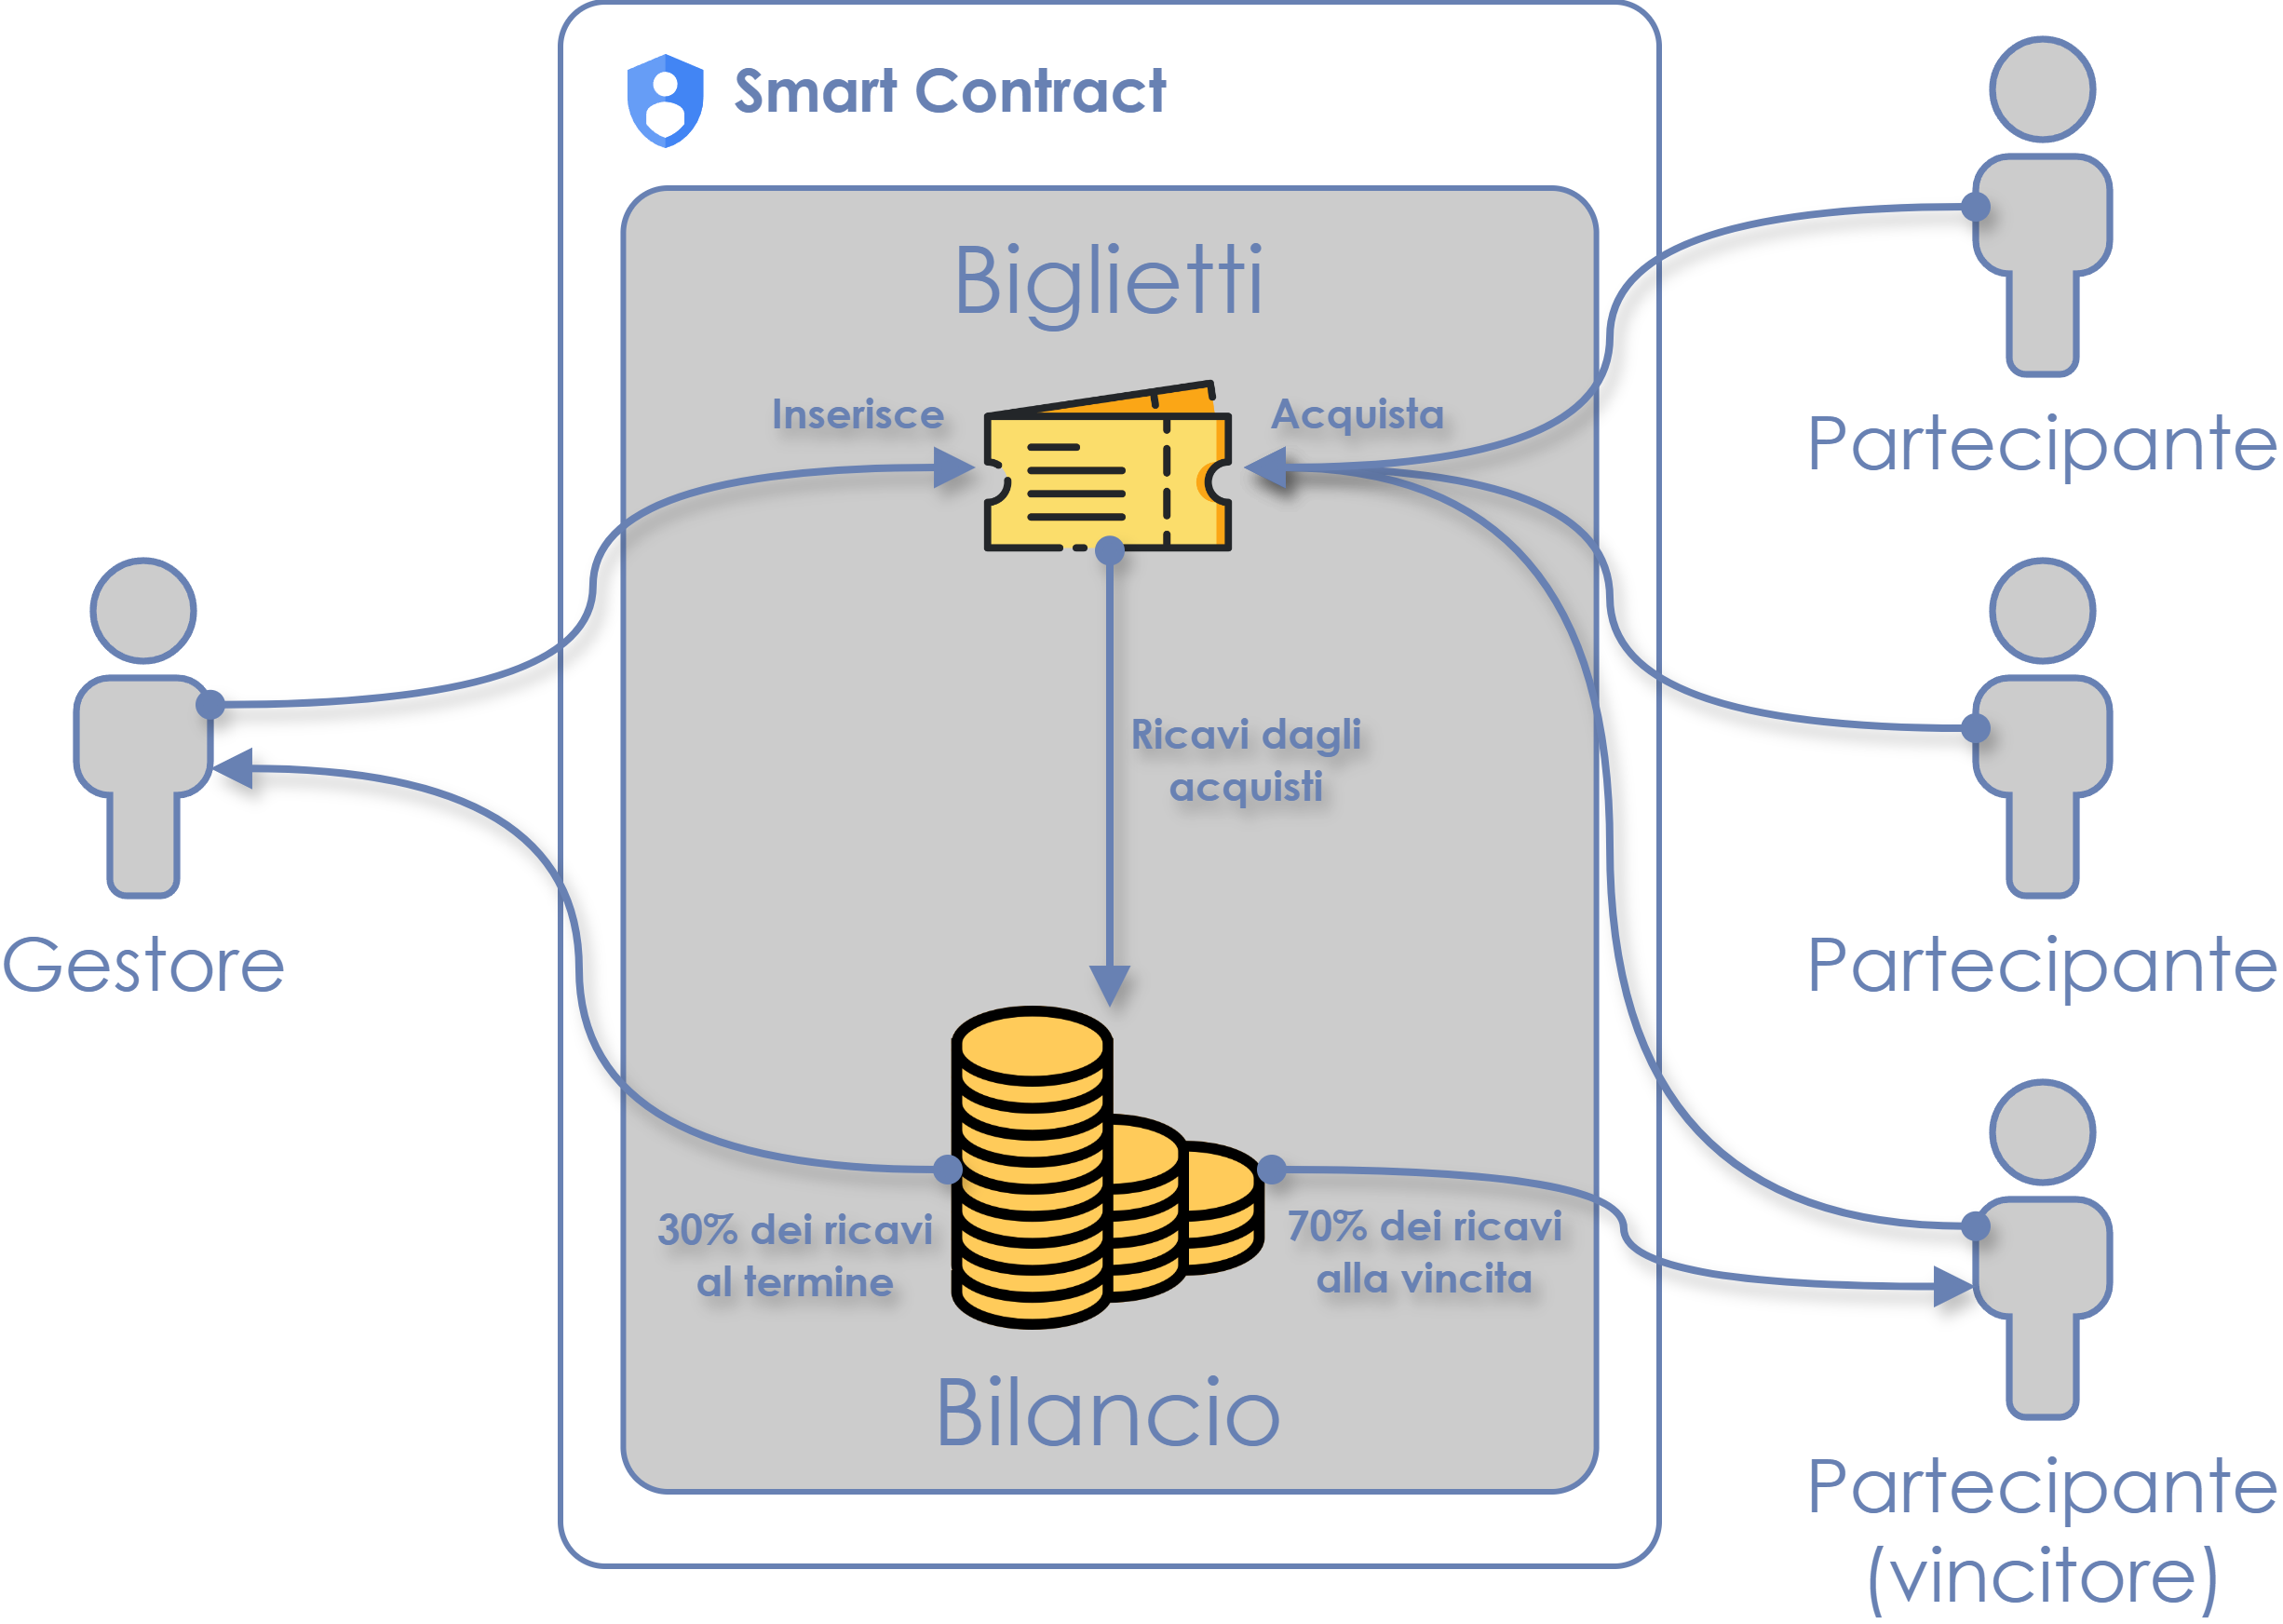
\includegraphics[width=\textwidth]{figures/my_app_diagram.png}
\caption[Schema dell'applicazione]{Schema del processo di lotteria e di pagamenti}\label{fig:app_diagram}
\end{center}
\end{figure}
\section{Progettazione dello Smart Contract}
Il codice dello smart contract deve quindi fornire tutte le funzioni necessarie per effettuare le operazioni sopra elencate. Il richiedente delle funzioni viene autenticato tramite il proprio indirizzo del ledger. La gestione del denaro è effettuata direttamente dallo smart contract, utilizzando il suo bilancio interno per immagazzinare e distribuire i token.\\
Come linguaggio per lo sviluppo è stato scelto \textit{Solidity}, un linguaggio di programmazione ideato per lo sviluppo di smart contract su Ethereum. Dato che la \acrshort{vm} di IOTA implementa il modello della \acrshort{evm} di Ethereum, gli smart contract scritti in questo linguaggio sono completamente compatibili anche con il ledger di IOTA. Per la compilazione del codice dello smart contract si è scelto di utilizzare \textit{Remix}, un IDE online che permette di programmare, compilare, fare il deploy e interagire con smart contract.\\
Il deploy viene effettuato su una \textit{testnet} di IOTA fornita dalla fondazione a scopi di test. Al suo interno è infatti possibile ottenere qualsiasi quantità di token IOTA fittizi tramite \textit{faucet}. Per collegarsi alla testnet viene utilizzato \textit{MetaMask}, un'estensione del browser che permette di connettersi a reti di ledger distribuiti e di creare e gestire wallet con multipli account. 
\newpage
\section{Progettazione dell'applicazione esterna}
L'applicazione esterna deve permettere agli utenti di interagire tramite interfaccia grafica con le funzioni dello smart contract, potendone modificare e visualizzare lo stato. È stato scelto di sviluppare un'applicazione web utilizzando \textit{React} e \textit{Typescript}. Come libreria per interfacciarsi alla rete di IOTA e allo smart contract sono state considerate sia \textit{ethers.js} che \textit{web3.js}. È stato infine scelto di utilizzare web3.js data la sua maggiore rilevanza storica e supporto sviluppato nel tempo. web3.js è infatti la prima e originale libreria per l'interazione con smart contract, sviluppata direttamente dalla fondazione Ethereum\footnote{\url{https://web3js.org/}}.\\ 
Tale libreria viene poi fatta interfacciare con MetaMask, utilizzandolo come provider (vedi \ref{connect_contract}) per collegarsi alla rete IOTA in cui è presente lo smart contract.\\
L'applicazione fornisce due schermate principali: la schermata gestore e la schermata partecipante.
\begin{description}[font=$\bullet$\:\:,leftmargin=\parindent,labelindent=\parindent]
  \item[Schermata gestore] La schermata visualizzata da chi ha creato la lotteria. Gli permette di interagire con tutte le funzioni di amministrazione e monitoraggio dello smart contract, e di ritirare i suoi guadagni una volta conclusa la lotteria.
  \item[Schermata partecipante] La schermata visualizzata da tutti gli altri utenti. Permette a un utente di partecipare alla lotteria acquistando un biglietto, e di ritirare la sua vincita in caso di vittoria.
\end{description}
È inoltre prevista una schermata iniziale di accesso, che permette la creazione di una nuova lotteria oppure l'accesso a una già esistente.\\
In Figura \ref{fig:interaction_diagram} è riportata la sequenza di operazioni dell'applicazione finale per richiamare le funzioni dello smart contract.

\begin{figure}[h]
\begin{center}
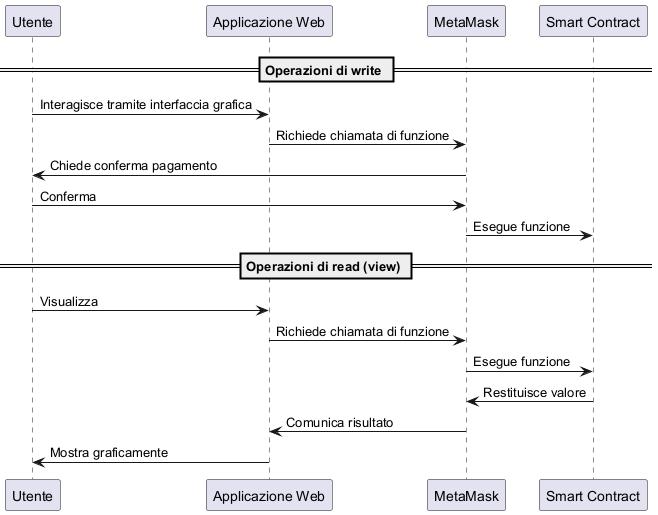
\includegraphics[width=\textwidth]{figures/my_interaction_diagram.png}
\caption[Diagramma delle interazioni]{Diagramma di sequenza sulle interazioni fra utente, applicazione web e smart contract}\label{fig:interaction_diagram}
\end{center}
\end{figure}


\clearpage{\pagestyle{empty}\cleardoublepage}



%%%%%%%%%%%%%%%%%%%%%%%%%%%%%%%%%%%%%%%%
% IMPLEMENTAZIONE
\chapter{Implementazione}
\label{chap:implementation}
% Come abbiamo implementato il programma, se ci sono state scelte particolari o punti particolarmente ostici che sono stati superati. Se ci sono state difficolt\`a insormontabili vanno spiegate.\\
% \`E necessario inserire estratti di codice, tabelle o immagini nella tesi solamente quando questi aiutano la comprensione dell'argomento. Se pensate di stare scrivendo una parte molto tecnica e poco comprensibile al lettore, aiutatevi con le immagini o con il codice. Per inserire estratti di codice rifarsi all'esempio seguente oppure \`e possibile usare il package  \href{https://www.overleaf.com/learn/latex/Code\_listing}{listing}.
% \begin{minted}{c}
% #include <stdio.h>
% int main() {
%    // printf() displays the string inside quotation
%    printf("Hello, World!");
%    return 0;
% }
% \end{minted}
In questo capitolo viene descritta nel dettaglio l'implementazione del progetto, analizzando le scelte tecniche effettuate e le difficoltà riscontrate. Il processo di implementazione è avvenuto creando una versione iniziale dello smart contract, per poi portare avanti il suo sviluppo in parallelo con quello dell'applicazione web, in base alle necessità riscontrate durante l'implementazione di quest'ultima.\\
La prima sezione è dedicata alla descrizione del processo di sviluppo dello smart contract, analizzando la logica di implementazione delle sue funzionalità e le soluzioni adottate per garantire efficienza e sicurezza.\\
Successivamente, viene illustrato lo sviluppo dell'applicazione web, soffermandosi sull'interazione con lo smart contract e sugli strumenti necessari per consentirla.\\
Il codice sviluppato per lo smart contract e per l'applicazione web è consultabile su GitHub\footnote{\url{https://github.com/UniboSecurityResearch/Paris_Manuel_BT}}, all'interno della cartella \texttt{project}.

\section{Implementazione dello Smart Contract}
Come appena introdotto, lo sviluppo dello smart contract ha seguito un processo di evoluzione graduale, portando allo sviluppo di più versioni del programma.
\begin{enumerate}[font=\bfseries]
    \item \textbf{La prima versione} implementava la struttura base del sistema di lotteria, senza l'integrazione del sistema di pagamento.
    \item \textbf{La seconda versione}, sviluppata subito dopo, incorporava nel sistema di lotteria il meccanismo di pagamento dei biglietti e di riscossione dei guadagni.
    \item \textbf{La terza ed ultima versione}, sviluppata in contemporanea con l'implementazione dell'applicativo web, include modifiche e aggiunte alle funzioni dello smart contract necessarie al corretto funzionamento dell'applicazione.
\end{enumerate}

\subsection{Prima versione: struttura base}
La prima fase di sviluppo è stata puramente dedicata a creare la struttura base dello smart contract e a renderlo funzionante e interagibile su blockchain. In questa versione un'entità può creare una lotteria effettuando il deploy dello smart contract, e può eseguire le funzioni amministrative e di monitoraggio elencate nel capitolo precedente. Un partecipante può ottenere un biglietto (senza effettuare un pagamento) e al termine della lotteria visualizzare se ha vinto.\\
I biglietti vengono memorizzati all'interno di un array \texttt{tickets} e sono identificati in due modi differenti:
\begin{enumerate}
    \item Un ID numerico, ossia il valore con cui un biglietto viene salvato nell'array. Questo viene utilizzato principalmente per distinguere graficamente i biglietti fra di loro.
    \item L'indice della posizione del biglietto nell'array. Questo è invece quello che viene utilizzato per identificare i biglietti nel codice. 
\end{enumerate}
Il biglietto vincente è identificato attraverso l'indice del biglietto nell'array, che viene memorizzato in una variabile \texttt{winning\_ticket\_id}. Lo stato della lotteria invece viene gestito tramite la variabile \texttt{is\_lottery\_open}, un booleano che indica se la lotteria è ancora aperta o se è stata chiusa dal gestore.\\
Un grande vantaggio della programmazione di smart contract è che essi rendono l'autenticazione un processo molto semplice da implementare e allo stesso tempo sicuro grazie al ledger. All'interno dello smart contract infatti, ciascuna entità viene autenticata tramite il proprio indirizzo nel ledger. Al deploy dello smart contract l'indirizzo del creatore viene registrato in una variabile chiamata \texttt{lottery\_manager}. Questa variabile sarà quella utilizzata nel codice per autenticare l'indirizzo del chiamante, verificando se coincide con quello del gestore della lotteria. Per autenticare un partecipante invece è utilizzato un mapping \texttt{participants} che associa un indirizzo a una struct \texttt{Participant}. Questa struct possiede i seguenti campi:
\begin{itemize}
    \item \texttt{ticket\_id}: indice della posizione nell'array del biglietto preso dal partecipante
    \item \texttt{got\_ticket}: booleano che indica se il partecipante ha preso un biglietto o meno. Questo campo è necessario poiché il semplice controllo che il campo \texttt{ticket\_id} non sia impostato, non è sufficiente. Il motivo è che la mappatura iniziale del mapping associa a un indirizzo una struct con variabili inizializzate a 0, in questo caso quindi \texttt{ticket\_id = 0} e \texttt{got\_ticket = false}. Non sarebbe quindi possibile effettuare il controllo su \texttt{ticket\_id} poiché il primo biglietto ha indice 0.
\end{itemize}
Sono stati inoltre definiti dei \textit{modificatori} per semplificare l'autenticazione e la sicurezza nel codice. In Solidity, un modificatore serve ad aggiungere dei controlli aggiuntivi ad una funzione. Applicando un modificatore ad una funzione, verranno prima effettuati i controlli previsti dal modificatore, e solo in caso di esito positivo viene eseguita la funzione.
Nel Codice \ref{lst:modifiers} è mostrato un esempio di come è stato applicato un modificatore nel codice.
\begin{lstlisting}[language=Solidity, caption=Utilizzo dei modificatori, label={lst:modifiers}]
// Dichiarazione del modificatore
modifier is_participant() {
    require(participants[msg.sender].got_ticket, "You didn't get a ticket yet.");
    _;
}
// Modificatore applicato alla funzione
function check_ticket() public view is_participant returns (uint) {
    Participant storage participant = participants[msg.sender];
    return (tickets[participant.ticket_id]);
}
\end{lstlisting}
In questo estratto di codice, viene definito il modificatore \texttt{is\_participant} che verifica che il chiamante sia un partecipante alla lotteria in possesso di un biglietto. Applicandolo alla funzione \texttt{check\_ticket} che restituisce il biglietto posseduto dal chiamante, la funzione restituirà soltanto se il chiamante è effettivamente in possesso di un biglietto, altrimenti fallirà l'esecuzione. La logica di esecuzione è che il corpo della funzione viene inserito nel modificatore al posto dell'apposito indicatore, qui specificato in riga 4. Viene poi eseguito il modificatore con all'interno il corpo della funzione.\\ 
I modificatori definiti per questo smart contract sono i seguenti:
\begin{itemize}
    \item \texttt{manager\_rights}: controlla che il chiamante sia il gestore della lotteria, comparando il suo indirizzo con quello salvato in \texttt{lottery\_manager}.
    \item \texttt{is\_participant}: come riportato nel Codice \ref{lst:modifiers}, controlla che il chiamante sia un partecipante attivo alla lotteria. In altre parole viene controllato che, tramite il mapping \texttt{participants}, l'indirizzo del chiamante sia associato ad un \texttt{Participant} con \texttt{got\_ticket = true}.
    \item \texttt{lottery\_open}: controlla che la lotteria sia ancora aperta, tramite l'omonima variabile.
    \item \texttt{lottery\_closed}: analogo al precedente, controllando l'inverso della variabile \texttt{lottery\_open}.
\end{itemize}

Di seguito sono invece descritti i metodi di implementazione delle funzionalità che deve svolgere lo smart contract.

\subsubsection{Deploy e creazione della lotteria}
Lo smart contract ha una funzione costruttore che viene chiamata al momento del deploy. È quindi quella che viene chiamata alla creazione della lotteria. Il costruttore prende in input i seguenti parametri:
\begin{itemize}
    \item \texttt{new\_tickets}: array contenente i biglietti iniziali della lotteria. A questo array sarà successivamente possibile aggiungere biglietti, ma non rimuoverne.
    \item \texttt{new\_winning\_ticket\_id}: indice corrispondente alla posizione del biglietto vincente nell'array, che potrà successivamente essere modificato.
\end{itemize}
Dopo aver verificato che l'indice fornito sia nel range di lunghezza dell'array, il costruttore assegna i parametri alle corrispondenti variabili dello smart contract: \texttt{tickets} e \texttt{winning\_ticket\_id}. Assegna poi alla variabile \texttt{lottery\_manager} il valore di \texttt{msg.sender}, che corrisponde all'indirizzo dell'attuale chiamante della funzione. In questo modo viene permanentemente registrato come gestore della lotteria colui che ha effettuato il deploy.

\subsubsection{Gestore: amministrazione della lotteria}
Per permettere al gestore della lotteria di eseguire le funzionalità di amministrazione e monitoraggio sono state definite le seguenti funzioni, che utilizzano tutte il modificatore \texttt{manager\_rights} in modo da poter essere chiamate soltanto dal gestore:
\begin{itemize}
    \item \texttt{close\_lottery}: permette di chiudere la lotteria impostando \texttt{is\_lottery\_open = false}. Utilizza anche il modificatore \texttt{lottery\_open} per fare in modo che la funzione sia chiamabile soltanto se la lotteria non è già stata chiusa.
    \item \texttt{add\_ticket}: permette di aggiungere un nuovo biglietto a quelli disponibili. Prende in input il parametro \texttt{new\_ticket} contenente l'ID numerico del biglietto, e ne esegue il push in \texttt{tickets}. Analogamente alla precedente funzione utilizza anche il modificatore \texttt{lottery\_open}.
    \item \texttt{change\_winning\_ticket}: permette di modificare l'indice del biglietto vincente. Prende in input il parametro \texttt{new\_winning\_ticket\_id} contenente il nuovo indice del biglietto vincente, che viene assegnato alla rispettiva variabile \texttt{winning\_ticket\_id}. Analogamente alle funzioni precedenti viene utilizzato il modificatore \texttt{lottery\_open}. È presente inoltre un controllo aggiuntivo in cui viene verificato che il nuovo indice sia valido, ovvero che rientri nella lunghezza massima dell'array \texttt{tickets}.
    \item \texttt{check\_tickets} \textit{(view)}: permette di visualizzare l'array di tutti i biglietti presenti nella lotteria, restituendo \texttt{tickets}.
    \item \texttt{check\_winning\_ticket} \textit{(view)}: permette di visualizzare l'indice del biglietto vincente, restituendo \texttt{winning\_ticket\_id}.
    \item \texttt{check\_ticket\_allotment} \textit{(view)}: permette di visualizzare il numero di biglietti venduti, restituendo la variabile \texttt{ticket\_allotment} (descritta nel prossimo paragrafo).
\end{itemize}

\subsubsection{Partecipante: ottenimento del biglietto e controllo della vincita}
Per permettere a un utente che vuole partecipare alla lotteria di acquisire un biglietto e verificare la vincita, sono state definite le seguenti funzioni:
\begin{itemize}
    \item \texttt{get\_ticket}: permette di ottenere un biglietto fra quelli disponibili. L'assegnazione dei biglietti è stata implementata in modo sequenziale. Viene per questo utilizzata una variabile \texttt{ticket\_allotment} inizializzata a 0 e incrementata ad ogni chiamata di questa funzione, che tiene traccia dell'indice del prossimo biglietto da assegnare\footnote{Allo stesso tempo, questa variabile corrisponde anche al numero di biglietti assegnati.}. Si utilizza quindi il mapping \texttt{participants} per ottenere l'istanza della struct \texttt{Participant} associata all'indirizzo del chiamante. Tale istanza viene impostata con \texttt{got\_ticket = true} e \texttt{ticket\_id = ticket\_allotment}. Dopodiché \texttt{ticket\_allotment} viene incrementata di 1 per la prossima assegnazione. Viene utilizzato il modificatore \texttt{lottery\_open} in modo da permettere l'acquisto solamente se la lotteria è aperta. Sono inoltre presenti i seguenti controlli aggiuntivi: 
    \begin{itemize}
        \item Il chiamante non può essere il gestore, \texttt{msg.sender} deve quindi essere diverso da \texttt{lottery\_manager}.
        \item Devono esserci ancora biglietti disponibili, \texttt{ticket\_allotment} deve quindi essere minore della lunghezza di \texttt{tickets}.
        \item Il chiamante non deve aver già acquistato un biglietto, il campo \texttt{got\_ticket} dell'istanza di \texttt{Participant} associata all'indirizzo \texttt{msg.sender} deve quindi essere \texttt{false}.
    \end{itemize}
    \item \texttt{check\_ticket} \textit{(view)}: come mostrato anche nel Codice \ref{lst:modifiers}, permette di visualizzare l'ID numerico del proprio biglietto. Restituisce quindi \texttt{tickets[ticket\_id]}, dove \texttt{ticket\_id} è l'indice del biglietto che è stato precedentemente assegnato al chiamante tramite \texttt{get\_ticket}. La funzione utilizza il modificatore \texttt{is\_participant} in modo da poter essere chiamata solo da chi possiede un biglietto.
    \item \texttt{check\_winning} \textit{(view)}: permette di visualizzare se il proprio biglietto è quello vincente. Restituisce quindi il booleano risultante da \texttt{ticket\_id == winning\_ticket\_id}, dove \texttt{ticket\_id} è l'indice del biglietto assegnato al chiamante. È utilizzato il modificatore \texttt{is\_participant}, analogo alla funzione precedente. È inoltre utilizzato il modificatore \texttt{lottery\_closed}, in modo da permettere di verificare la vincita solo se la lotteria è stata chiusa. 
\end{itemize}

\subsection{Seconda versione: acquisti e pagamenti}
Dopo aver portato a termine la prima versione completa dello smart contract e aver testato le sue varie componenti in modo che fosse tutto funzionante, è cominciato lo sviluppo della seconda versione. Questa versione, come introdotto prima, introduce nello smart contract il sistema di pagamento. Diventa quindi necessario pagare un prezzo fisso per l'acquisto di un biglietto, e alla fine della lotteria vengono distribuiti pagamenti al gestore e al vincitore della lotteria. Come introdotto nel capitolo precedente, è stato deciso un prezzo di 10 IOTA per l'acquisto di un biglietto, e una retribuzione per il gestore e per il vincitore di rispettivamente il 30\% e il 70\% dei guadagni totali dalle vendite dei biglietti. Sono stati scelti dei valori in modo che risultassero sempre numeri interi nella divisione dei guadagni, poiché una limitazione dello smart contract è che non può gestire numeri float.\\
I metodi di implementazione del sistema di pagamento sono descritti qui di seguito.
\subsubsection{Pagamento dall'utente allo smart contract}
I pagamenti effettuati dall'utente verso lo smart contract, ovvero gli acquisti dei biglietti, vengono effettuati direttamente tramite la transazione stessa. Questo significa che, quando l'utente chiama la funzione per acquistare il biglietto, inserisce la somma necessaria nella stessa transazione che contiene la chiamata. Il pagamento viene ricevuto automaticamente dallo smart contract, che verifica poi se la quantità di denaro fornita è adeguata. In caso contrario, viene annullata la chiamata e restituito il denaro.
\subsubsection{Pagamento dallo smart contract all'utente}
Per effettuare dei pagamenti dall'interno dello smart contract, in Solidity sono disponibili tre diverse funzioni, comparate qui di seguito in Tabella \ref{tab:pay_functions}.
\newpage
\begin{center}
\begin{longtable}{c|m{0.25\linewidth}|m{0.25\linewidth}|m{0.25\linewidth}}
\textbf{Funzione} & \textbf{Valore restituito} & \textbf{Gas utilizzato} & \textbf{Funzionalità \linebreak aggiuntive}\\
\hline \hline
\texttt{transfer} & Niente in caso di successo, lancia un errore in caso di fallimento. & 2300 gas & Nessuna\\
\hline
\texttt{send} & \texttt{true} in caso di successo, \texttt{false} in caso di fallimento. & 2300 gas & Nessuna\\
\hline
\texttt{call} & \texttt{true} in caso di successo, \texttt{false} in caso di fallimento\footnote{Quando si utilizza per chiamare funzioni di altri smart contract, restituisce un parametro aggiuntivo contenente l'output della chiamata.}. & Si adatta dinamicamente al gas necessario per la chiamata e non ha limiti. & Permette anche di chiamare funzioni di altri smart contract.\\
\hline \hline
\caption[Funzioni di pagamento]{Funzioni di pagamento in Solidity\footnotemark}\label{tab:pay_functions}
\end{longtable}
\end{center}
\footnotetext{\href{https://dev.to/ceasermikes002/understanding-send-transfer-and-call-in-solidity-security-implications-and-preferences-4pog}{\texttt{https://dev.to/ceasermikes002/understanding-send-transfer-and-call-in- solidity-security-implications-and-preferences-4pog}}}
La funzione scelta per implementare i pagamenti dallo smart contract all'utente in questo progetto è \texttt{call}. Tale funzione è quella attualmente più utilizzata, data la sua flessibilità e la sua gestione dinamica e senza limiti del gas. Questo introduce però allo stesso tempo anche dei rischi nell'utilizzo, se non viene gestita con i dovuti accertamenti. Non avendo infatti limiti di gas e permettendo anche di chiamare funzioni di altri smart contract, c'è un rischio di abuso da parte del ricevente. Se il ricevente è uno smart contract, potrebbe infatti chiamare più volte ricorsivamente la funzione del nostro smart contract che lancia la \texttt{call}, ricevendo così il pagamento multiple volte. Per evitare questo comportamento è necessario strutturare la funzione in modo che \textit{prima} vengano effettuati i controlli e le modifiche allo stato, e come ultima operazione la \texttt{call}. Un esempio del corretto utilizzo è mostrato nel Codice \ref{lst:call}, che riporta l'implementazione della funzione di pagamento al vincitore (descritta successivamente in \ref{cash_in}).
\begin{lstlisting}[language=Solidity, caption=Corretto utilizzo di \texttt{call}, label={lst:call}]
function cash_in_victory() public is_participant lottery_closed {
    // Controlli
    Participant storage participant = participants[msg.sender];
    require(participant.ticket_id == winning_ticket_id, "Your ticket is not the winning ticket");
    require(!cashed_in, "Winning already cashed in.");
    if(earnings_retrieved)
        winning_amount = address(this).balance;
    else
        winning_amount = (address(this).balance * 7) / 10;  
    // Modifiche allo stato
    cashed_in = true;
    // Pagamento con call
    (bool success, ) = payable(msg.sender).call{value: winning_amount}("");
    require(success, "Error cashing in");
}
\end{lstlisting}
In questo modo, anche se tramite la \texttt{call} uno smart contract ricevente dovesse nuovamente chiamare \texttt{cash\_in\_victory} prima che termini, la seconda chiamata non andrebbe mai a buon fine. Questo perché, come prima cosa, la funzione controlla che il campo \texttt{cashed\_in} non sia \texttt{true} (riga 5), valore che viene impostato \textit{prima} del lancio di \texttt{call}\footnote{Se venisse impostato dopo, il ricevente potrebbe richiamare \texttt{cash\_in\_victory} e ricevere nuovamente un pagamento prima che venga impostato \texttt{cashed\_in = true}.} (riga 11). Inoltre, essendo \texttt{call} priva di un lancio automatico di errore in caso di fallimento, è necessario gestirlo automaticamente tramite il booleano restituito dalla funzione (riga 14).

\subsubsection{Aggiunte alle funzioni dello smart contract}
Per implementare il pagamento dei biglietti, sono state effettuate le seguenti modifiche alla funzione \texttt{get\_ticket}:
\begin{itemize}\label{contract_payments}
    \item È stata adeguatamente rinominata in \texttt{buy\_ticket}.
    \item È stata resa una funzione \texttt{payable}. È grazie a questo che lo smart contract può ricevere dei pagamenti attraverso la transazione di chiamata a questa funzione.
    \item È stato aggiunto un controllo aggiuntivo che richiede un pagamento tramite la transazione di chiamata di esattamente 10 IOTA. Tale valore è verificabile in \texttt{msg.value}. In Solidity, l'unità utilizzata dallo smart contract per gestire i bilanci è \textit{Wei}\footnote{Una sottounità di Ether, la valuta di Ethereum. 1 Wei equivale a \(10^{-18}\) Ether.}. È stato quindi necessario, nel controllo che verifica il valore del pagamento, specificare \texttt{10 ether}\footnote{La specifica è in Ether e non in IOTA perché Solidity è un linguaggio inizialmente sviluppato per Ethereum. In una blockchain IOTA, la valuta Ether nel codice viene considerata come IOTA.}. 
    \end{itemize}
\label{close_lottery}Inoltre, è stato aggiunto un controllo aggiuntivo alla funzione \texttt{close\_lottery}, che permette la chiusura della lotteria soltanto con le seguenti condizioni:
\begin{itemize}
    \item Nessun biglietto è ancora stato venduto. In questo caso la lotteria viene considerata annullata.
    \item Se dei biglietti sono stati venduti, allora è necessario che ne siano stati venduti almeno due e che il biglietto vincente sia fra quelli venduti. La prima condizione è necessaria per fare in modo che il vincitore della lotteria abbia un guadagno dalla vincita. Se infatti viene chiusa la lotteria con soltanto un biglietto acquistato, il possessore riceverà una vincita pari al 70\% del prezzo dell'unico biglietto, finendo quindi per perdere il 30\% di ciò che ha pagato. La seconda condizione è invece necessaria per evitare frodi da parte del gestore, assicurandosi che la lotteria non venga chiusa senza che il biglietto vincente sia stato venduto a qualcuno.
\end{itemize}
Sono infine state aggiunte le seguenti funzioni per permettere la riscossione dei guadagni da parte del gestore e del vincitore:
\begin{itemize}
    \item \label{cash_in}\texttt{cash\_in\_victory}: mostrata anche nel Codice \ref{lst:call}, questa funzione permette al vincitore della lotteria di riscattare la sua vincita. Controlla innanzitutto che il chiamante sia effettivamente il vincitore, comparando il campo \texttt{ticket\_id} del \texttt{Participant} associato al chiamante con la variabile \texttt{winning\_ticket\_id} dello smart contract. Verifica poi che il vincitore non abbia già riscattato la sua vincita, utilizzando una variabile booleana \texttt{cashed\_in} inizializzata a \texttt{false}. In questo modo vengono impedite riscossioni multiple del denaro. Dopodiché, per decidere la quantità di bilancio dello smart contract da pagare al vincitore, viene controllato se il gestore ha già riscattato i suoi guadagni. Questo avviene tramite una variabile booleana \texttt{earnings\_retrieved} inizializzata a \texttt{false}, analoga a \texttt{cashed\_in} ma relativa al gestore. Se li ha già riscattati, al vincitore spetta tutta la parte rimanente del bilancio dello smart contract, altrimenti il 70\%. In seguito ai controlli e prima di inviare il denaro, viene impostata \texttt{cashed\_in = true}. Infine, viene lanciata l'effettiva \texttt{call} all'indirizzo di \texttt{msg.sender}, specificandolo come indirizzo \texttt{payable}, inviando la quantità di token appena calcolata. Verifica poi che il pagamento sia andato a buon fine, effettuando il revert della funzione in caso contrario. Questa funzione utilizza i modificatori \texttt{is\_participant} e \texttt{lottery\_closed}, in modo da permetterne la chiamata solo da chi possiede un biglietto e se la lotteria è già stata chiusa.
    \item \texttt{retrieve\_earnings}: permette al gestore della lotteria di riscattare i suoi guadagni. Il funzionamento è speculare a \texttt{cash\_in\_victory} invertendo \texttt{cashed\_in} e \texttt{earnings\_retrieved}, e inviando una quantità di token del 30\% dei ricavi invece che del 70\%. Utilizza i modificatori \texttt{manager\_rights} e \texttt{lottery\_closed}, in modo da poter essere chiamata solo dal gestore dopo il termine della lotteria. 
\end{itemize}

\subsection{Terza versione: integrazione con l'applicativo}
Mentre le prime due versioni dello smart contract sono state sviluppate in modo autonomo rispetto all'applicazione web, la terza ed ultima versione è stata elaborata in contemporanea ad essa. Questo perché, incominciando l'effettivo sviluppo dell'applicazione web e delle sue interazioni con lo smart contract, si sono presentate necessità aggiuntive per lo smart contract che non erano state considerate durante il suo sviluppo autonomo. Durante lo sviluppo dello smart contract infatti, le funzioni venivano provate tramite l'interfaccia di Remix, che permette di visualizzare gli errori delle chiamate. Tali errori, come ad esempio quelli dati dai modificatori o da altri controlli aggiunti, venivano mostrati e differenziati fra loro senza problemi. Questo però, effettuato in un'applicazione destinata all'uso reale, non è ottimale in quanto viene sprecata una transazione che viene poi annullata a causa dell'errore. Questo causa infatti anche dei problemi quando si utilizza MetaMask per confermare la transazione, in quanto MetaMask calcola una stima di gas errata e molto elevata quando prevede che la transazione fallirà. Inoltre, gli errori personalizzati dello smart contract sono più difficili da catturare e gestire separatamente all'interno dell'applicazione esterna. Sono state quindi necessarie delle view aggiuntive per permettere all'applicazione, quando possibile, di fare i controlli \textit{prima} di chiamare le funzioni. In questo modo è possibile impedire le chiamate a priori senza far scattare degli errori. Inoltre, ulteriori view sono state aggiunte anche per necessità grafiche e di controlli interni riscontrate nella creazione del layout dell'applicazione web, in modo da permettere agli utenti di visualizzare adeguatamente tutte le informazioni necessarie.\\
Le view aggiunte allo smart contract in questa versione finale sono le seguenti:
\begin{itemize}\label{uuid}
    \item \texttt{check\_ticket\_availability}: restituisce un booleano che indica se ci sono ancora biglietti disponibili o se sono esauriti. Per farlo controlla se la variabile \texttt{ticket\_allotment}, equivalente al numero di biglietti venduti, è minore della lunghezza di \texttt{tickets}. Non utilizza nessun modificatore ed è quindi chiamabile in qualsiasi situazione. Questa view è stata definita per permettere all'applicativo di controllare se ci sono ancora biglietti disponibili all'acquisto, prima di permettere di richiamare la funzione \texttt{buy\_ticket}.
    \item \texttt{check\_UUID}: definita in contemporanea a una nuova costante \texttt{contract\_UUID} dello smart contract, contenente un UUID immutabile che identifica un'istanza di questo smart contract. Questa view prende in input il parametro \texttt{uuid} e confronta il suo hash\footnote{Ottenuto tramite \texttt{keccak256(abi.encodePacked(uuid))}} con quello della costante \texttt{contract\_UUID}. Restituisce poi un booleano in base al risultato. Questa view è stata definita per permettere all'applicativo, quando l'utente prova ad accedere a una lotteria, di verificare che l'indirizzo fornito sia dell'istanza di uno smart contract lotteria. In questo modo, se tramite l'applicazione si tentasse di inserire l'indirizzo di uno smart contract che non è un'istanza lotteria, la chiamata a \texttt{check\_UUID} non andrebbe a buon fine\footnote{Sia nel caso in cui la funzione non esista in quello smart contract, sia nell'eventualità in cui invece esista. È infatti quasi completamente impossibile che utilizzi lo stesso UUID.} e permetterebbe all'applicazione di gestire correttamente la cosa.
\end{itemize}
Sono inoltre state create anche delle variabili pubbliche aggiuntive, per memorizzare ulteriori dati necessari all'interfaccia grafica:
\begin{itemize}
    \item \texttt{winning\_amount}: memorizza la somma di denaro guadagnata dal vincitore. Questo avviene al momento della chiamata di \texttt{cash\_in\_victory}. È stata definita per permettere all'applicativo di mostrare graficamente al vincitore quanti IOTA ha vinto al momento del riscatto della vincita.
    \item \texttt{earned\_amount}: analoga alla precedente, ma per la somma guadagnata dal gestore della lotteria.
    \item \texttt{lottery\_name}: implementa la possibilità di dare un nome alla lotteria al momento della creazione. Questa variabile viene infatti registrata tramite un nuovo parametro \texttt{new\_lottery\_name} della funzione costruttore dello smart contract. È stata definita per permettere all'applicazione di visualizzare graficamente un nominativo per l'attuale lotteria, in modo da poter riconoscere a quale si sta partecipando nella schermata attuale.
\end{itemize}
Tali variabili non necessitano della creazione esplicita di una view che le restituisca, poiché per le variabili pubbliche viene automaticamente generata una view con l'omonimo nome. Rendere delle variabili pubbliche è quindi utile quando si necessita di una view che restituisca la singola variabile e che non richieda alcuna restrizione sul suo utilizzo. Per lo stesso motivo, alcune variabili che prima erano private e utilizzate solo per controlli interni al codice, in questa versione sono state rese pubbliche per permetterne la creazione di una view:
\begin{itemize}
    \item \texttt{lottery\_manager}: resa pubblica per permettere all'applicativo di comparare l'indirizzo dell'utente connesso e verificare se è il gestore della lotteria. In questo modo l'applicazione può decidere quale schermata mostrare all'utente.
    \item \texttt{is\_lottery\_open}: resa pubblica per permettere all'applicativo di mostrare graficamente lo stato della lotteria, e di controllare quali funzioni mostrare all'utente in base a quali è permesso effettuare nello stato attuale.
    \item \texttt{cashed\_in}: resa pubblica per permettere all'applicativo di controllare se l'utente può richiamare la funzione \texttt{cash\_in\_victory} o se l'ha già fatto.
    \item \texttt{earnings\_retrieved}: resa pubblica per permettere all'applicativo di controllare se il gestore può richiamare la funzione \texttt{retrieve\_earnings} o se l'ha già fatto.
\end{itemize}
Un'altra implementazione che si è rivelata necessaria per la corretta integrazione con l'interfaccia grafica sono gli \textit{eventi}. In Solidity, un evento è un segnale che viene emesso dallo smart contract in determinati punti dell'esecuzione del codice. Chiunque sia in ascolto di tali segnali, in questo caso l'applicazione web, può catturarli e gestirli in tempo reale. Sono stati quindi implementati per permettere all'applicazione di aggiornarsi in tempo reale in contemporanea a determinati cambiamenti dello stato dello smart contract. Nel Codice \ref{lst:events} è mostrato un esempio di implementazione di evento.
\begin{lstlisting}[language=Solidity, caption=Utilizzo degli eventi, label={lst:events}]
// Dichiarazione dell'evento
event ticket_published(uint ticket);
// Emissione dell'evento in una funzione
function add_ticket(uint new_ticket) public manager_rights lottery_open {
    tickets.push(new_ticket);
    emit ticket_published(new_ticket);
}
\end{lstlisting}
In questo estratto di codice, viene dichiarato l'evento \texttt{ticket\_published} che prende in input il parametro \texttt{ticket}. Alla fine della funzione \texttt{add\_ticket} viene emesso tale evento, utilizzando il biglietto appena aggiunto come input. In questo modo, chiunque sia in ascolto dell'evento \texttt{ticket\_published} di questo smart contract, ogni volta che viene aggiunto un nuovo biglietto alla lotteria riceverà un segnale in tempo reale contenente l'identificativo numerico del biglietto.\\
Di seguito sono riportati gli eventi implementati nello smart contract:
\begin{itemize}
    \item \texttt{closed\_lottery}: viene emesso quando il gestore chiude la lotteria tramite \texttt{close\_lottery}. È stato implementato per permettere all'applicativo di aggiornare in tempo reale i controlli relativi a quali funzioni sono chiamabili nello stato attuale della lotteria. Se non ci fosse questo evento e il gestore chiudesse la lotteria mentre un utente sta visualizzando l'interfaccia dell'applicazione, l'interfaccia non si aggiornerebbe e all'utente sarebbe ad esempio permesso di chiamare la funzione per acquistare un biglietto, finendo per effettuare una transazione fallita.
    \item \texttt{ticket\_published}: come visto nel Codice \ref{lst:events}, viene emesso quando il gestore aggiunge un nuovo biglietto tramite \texttt{add\_ticket}. È stato implementato per permettere all'applicativo di notificare in tempo reale gli utenti quando viene aggiunto un nuovo biglietto, e per aggiornare i controlli relativi ai biglietti disponibili. Se infatti i biglietti erano precedentemente esauriti, alla ricezione di questo evento è possibile rieffettuare il controllo per permettere nuovamente all'utente di chiamare la funzione \texttt{buy\_ticket}.
    \item \texttt{ticket\_registered}: viene emesso quando un utente acquista un biglietto tramite \texttt{buy\_ticket}. Prende in input due parametri: \texttt{participant}, l'indirizzo di chi ha acquistato il biglietto, e \texttt{ticket}, l'identificativo numerico del biglietto. È stato implementato per permettere all'applicativo di notificare in tempo reale gli altri utenti quando qualcuno acquista un biglietto, e per aggiornare i controlli in modo analogo a \texttt{ticket\_published}. L'assenza di questo evento potrebbe portare al tentativo di acquisto di un biglietto quando sono invece esauriti, risultando in una transazione fallita.
\end{itemize}
\section{Implementazione dell'applicazione web}
Il processo di sviluppo dell'applicazione web consiste invece in un'iniziale implementazione delle due schermate gestore e partecipante, che si concentra principalmente sul collegare correttamente l'applicazione allo smart contract. Durante questa fase di sviluppo viene usato un unico smart contract lotteria, effettuandone il deploy manualmente da Remix e inserendolo nel codice come costante. Successivamente viene sviluppata anche una schermata di accesso che permette di creare un'istanza dello smart contract direttamente dall'applicativo, o di connettersi a un'istanza esistente tramite il suo indirizzo.

\subsection{Connessione allo Smart Contract}
La prima parte dello sviluppo dell'applicativo web è stata dedicata interamente a implementare la comunicazione con lo smart contract. È stata quindi innanzitutto creata un'interfaccia grafica minimale che permettesse di richiamare le funzioni dello smart contract in modo semplice. Come descritto nel capitolo precedente, il framework scelto per lo sviluppo dell'applicazione web è React. È stato quindi creato un progetto di base React con dei \texttt{Button} che potessero essere usati per chiamare le varie funzioni dello smart contract.\\
Per far comunicare l'applicazione con uno smart contract presente su blockchain si sono rivelati necessari i seguenti quattro componenti:
\begin{enumerate}[font=\bfseries]\label{connect_contract}
    \item \textbf{Un provider}, ovvero un collegamento che mette in comunicazione l’applicazione con la rete della blockchain, permettendo di inserire transazioni e ottenere dati dai suoi smart contract. Per le prime prove è stato utilizzato direttamente l'URL del provider della testnet IOTA fornito dalla fondazione.
    \item \textbf{L'indirizzo dello smart contract}. Tale indirizzo è quello con cui è identificata un'istanza di uno smart contract su una chain quando ne viene effettuato il deploy. Come introdotto precedentemente, in questa prima fase di sviluppo è stato inserito nel codice come costante \texttt{contractAddress}, ottenendolo direttamente da Remix dopo aver effettuato il deploy. 
    \item \textbf{L'\acrshort{abi} dello smart contract}. L'\acrfull{abi} è un json contenente
    l’interfaccia di tutte le variabili e funzioni dello smart contract, compresi gli input, gli output e i loro tipi. È necessario ad applicazioni esterne in modo da poter comunicare con lo smart contract e richiamare le sue funzioni, e può essere ottenuto dopo aver compilato il codice dello smart contract su Remix. Una volta fatto ciò è stato inserito nel progetto in un file \texttt{abi.json} che viene incluso nel file principale come costante \texttt{abi}. Nel Codice \ref{lst:abi} è riportato un esempio di come viene rappresentata una funzione all'interno dell'\acrshort{abi}, prendendo come campione la funzione \texttt{check\_UUID}.
    \item \textbf{Un collegamento a un account sul ledger}. Per le prime prove è stato inizialmente implementato inserendo nel codice la chiave privata dell'account come costante. Tale approccio, oltre a fissare l'account nel codice non permettendo a un utente di utilizzare il proprio, utilizza dati sensibili come la chiave privata e non avvisa l'utente nel momento in cui esegue operazioni che richiedono pagamenti.
\end{enumerate}
\begin{lstlisting}[language=Java, caption=Interfaccia di funzione nell'\acrshort{abi}, label={lst:abi}]
"inputs": [
    {
        "internalType": "string",
        "name": "uuid",
        "type": "string"
    }
],
"name": "check_UUID",
"outputs": [
    {
        "internalType": "bool",
        "name": "",
        "type": "bool"
    }
],
"stateMutability": "view",
"type": "function"
\end{lstlisting}
\label{connect_metamask}Come provider e collegamento agli account è stato successivamente implementato MetaMask come pianificato nel capitolo precedente. È stato quindi collegato MetaMask all'applicazione per essere utilizzato come provider. Tramite l'oggetto \texttt{window.ethereum} infatti, è possibile accedere al provider utilizzato dal browser dell'utente\footnote{Per verificare che tale provider sia MetaMask, è presente la variabile booleana \texttt{window.ethereum.isMetaMask}}. Per connettersi effettivamente a MetaMask si usa la funzione \texttt{window.ethereum.request({ method: 'eth\_requestAccounts' })}, che fornisce anche una lista contenente gli indirizzi degli account attualmente connessi a MetaMask. Il primo indirizzo della lista è quello attualmente attivo su MetaMask, e nell'applicazione viene quindi salvato in uno stato di React nominato \texttt{account}. In questo modo, MetaMask viene allo stesso tempo utilizzato anche come collegamento agli account, permettendo all'applicazione di interagire con lo smart contract tramite l'account dell'utente su MetaMask, senza richiedere dati aggiuntivi. Inoltre, sempre tramite MetaMask, l'utente è avvisato prima di compiere operazioni che richiedono pagamenti.\\
Una volta soddisfatti tutti i requisiti, è stato possibile collegarsi allo smart contract presente sulla blockchain utilizzando la libreria web3.js. Tramite \texttt{const web3 = new Web3(window.ethereum)} è stato creato l'oggetto Web3 utilizzando MetaMask come provider, e successivamente con \texttt{const contract = new web3.eth.Contract(abi, contractAddress)} viene creato l'oggetto tramite il quale si può comunicare con lo smart contract richiamando le sue funzioni. Vengono utilizzati due metodi per chiamare le funzioni dello smart contract, a seconda che siano funzioni view o funzioni di write:
\begin{enumerate}\label{app_payments}
    \item Per le funzioni view, si utilizza:
    \begin{minted}{java}
    contract.methods.<nome_funzione>(<parametri_funzione>)
    .call({ from: account })
    \end{minted} 
    Questa chiamata restituisce una \texttt{Promise} contenente i valori di ritorno della funzione dello smart contract. Non essendo funzioni che richiedono consumo di gas, MetaMask non richiede alcuna conferma per utilizzarle.
    \item Per le funzioni write invece, è stato inizialmente riscontrato un problema riguardo all'utilizzo del gas. Si è rivelato neccessario infatti, alla chiamata di una funzione, fornire come parametro anche una stima del gas utilizzato, in modo da pagare la quantità adeguata di tasse quando si conferma la transazione da MetaMask. Dopo vari tentativi falliti di stima del gas, anche tramite varie funzioni di web3.js, è stata infine trovata una funzione in grado di stimarlo correttamente ogni volta: \texttt{web3.eth.getGasPrice()}. Una volta stimato correttamente il gas tramite questa funzione, per chiamare funzioni write dello smart contract si utilizza:
    \begin{minted}{java}
    contract.methods.<nome_funzione>(<parametri_funzione>)
    .send({from: account, gasPrice: gasPrice})
    \end{minted}
    Per inserire un pagamento nella transazione della chiamata, come ad esempio per chiamare la funzione \texttt{buy\_ticket}, bisogna aggiungere a \texttt{send} un parametro aggiuntivo \texttt{value}. Dato che lo smart contract gestisce i bilanci in Wei (vedi \ref{contract_payments}), è necessario convertire il valore in tale unità. Sempre nel caso della funzione \texttt{buy\_ticket} che richiede un pagamento di 10 IOTA, si è convertito il valore in Wei con il metodo \texttt{web3.utils.toWei(10, "ether")}\footnote{Così come con Solidity, anche web3 è una libreria pensata per Ethereum. Allo stesso modo, l'unità Ether viene considerata come IOTA.}.\\
    Questa chiamata restituisce una Promise contenente l'hash della transazione effettuata. Prima di inviare la richiesta allo smart contract, viene chiesta conferma all'utente tramite MetaMask, specificando quanti IOTA dovrà spendere per effettuare la transazione.
\end{enumerate}
Una volta definite nel file le varie funzioni che richiamassero quelle dello smart contract, è stato sufficiente assegnarle agli \texttt{onClick} dei \texttt{Button} creati inizialmente per verificarne il funzionamento corretto.\\
L'ultima funzionalità dello smart contract da implementare nell'applicazione sono gli eventi. Durante tale implementazione sono stati riscontrati alcuni problemi e limitazioni. La prima limitazione è stata relativa all'utilizzo di MetaMask come provider, poiché non permette l'ascolto di eventi in tempo reale. Questo perché MetaMask è un provider HTTP, ovvero comunica con la chain tramite semplici chiamate e risposte HTTP. Per ascoltare gli eventi è necessario invece un provider WebSocket, che fornisce una connessione costante alla blockchain capace anche di ascoltare gli eventi in tempo reale\footnote{\url{https://metana.io/blog/what-are-web3-js-providers-explained/}}. È stato quindi necessario implementare un secondo provider parallelo a MetaMask, utilizzato esclusivamente per l'ascolto di eventi. Il provider WebSocket, connesso alla blockchain tramite l'URL della testnet di IOTA, è stato creato nel seguente modo:
\begin{minted}{java}
    const websocket = new Web3.providers.WebsocketProvider(
    "wss://ws.json-rpc.evm.testnet.iotaledger.net")
\end{minted}
Tramite il quale vengono creati i relativi oggetti Web3 con \texttt{const web3\_wss = new Web3(websocket)} e Contract con \texttt{const contract\_wss = new web3\_wss.eth.Contract(abi, contractAddress)}.\\
In questo modo, è stato infine possibile ascoltare in tempo reale gli eventi emessi dallo smart contract tramite la definizione di un listener relativo a ogni evento. Nel Codice \ref{lst:events_callback} è riportato un esempio di creazione di un listener, in cui viene gestito l'evento \texttt{ticket\_registered} nell'applicazione finale, emesso quando un utente acquista un biglietto.
\begin{lstlisting}[language=JSX, caption=Ricezione di un evento dello Smart Contract, label={lst:events_callback}]
    contract_wss.events.ticket_registered()
    .on("data", async (event) => { 
        // Gestione evento
        setLastTicketBought({
            participant: event.returnValues.participant, 
            ticket: event.returnValues.ticket
        })
    }) 
\end{lstlisting}
In questo estratto di codice, viene creato un listener per la callback \texttt{data} dell'evento, che viene attivata ogni volta che l'evento viene emesso dallo smart contract e rilevato dal listener. Viene ricevuto un oggetto \texttt{event}, che all'interno di \texttt{event.returnValues} contiene gli output dell'evento. Per testare inizialmente che gli eventi venissero ricevuti correttamente dall'applicazione, sono stati emessi esternamente\footnote{Tramite Remix, oppure tramite un'altra istanza dell'applicazione, ad esempio da un altro browser.} e mostrati nell'applicazione tramite \texttt{alert} nei listener.\\
\label{events_limitation}Un altro problema sorto relativo agli eventi riguarda il tempismo della ricezione. Si è riscontrato infatti che alcuni eventi vengono ricevuti dall'applicazione \textit{prima} che lo smart contract finisca l'esecuzione e aggiorni il suo stato. In questo caso quindi, la ricezione dell'evento dall'applicazione avviene troppo presto e non viene rilevato il nuovo stato, impedendo l'aggiornamento in tempo reale. Non è stato possibile eliminare completamente questa limitazione, ma è stata aggirata implementando un timeout di alcuni secondi per la gestione degli eventi emessi da funzioni che richiedono troppo tempo per aggiornare lo stato. Viene quindi utilizzato \texttt{new Promise(resolve => setTimeout(resolve, ms))} per creare un'attesa di \texttt{ms} millisecondi prima di gestire l'evento ricevuto.

\subsection{Sviluppo delle schermate gestore e partecipante}
Dopo che l'applicazione si è rilevata capace di comunicare correttamente con lo smart contract sulla blockchain potendo utilizzare tutte le sue funzionalità, si è conclusa la fase di test ed è iniziato lo sviluppo del layout dell'applicazione. Come già indicato in precedenza, questa fase di sviluppo consente all'applicazione di interagire con un unico smart contract già presente sulla blockchain, del quale viene inserito l'indirizzo in una costante \texttt{contractAddress}.\\ 
È stato definito il file principale \texttt{Lottery.jsx} che funge da contenitore generale per intercambiare le varie schermate.\\
Per creare il layout grafico sono stati utilizzati i seguenti moduli npm:
\begin{itemize}
    \item \textit{react-bootstrap}, che permette l'utilizzo delle classi CSS di bootstrap e fornisce inoltre dei componenti React pre-stilizzati.
    \item \textit{react-toastify}, che fornisce un componente React per la visualizzazione di notifiche stilizzabili.
\end{itemize}
La prima cosa che viene visualizzata quando si accede alla pagina di \texttt{Lottery.jsx} è un componente, definito nel file \texttt{NoMetamask.jsx}, che fornisce all'utente un \texttt{Button} per connettere l'applicazione a MetaMask, oppure lo informa in caso il browser attuale non supporti o non utilizzi MetaMask. Una volta connesso MetaMask con il metodo descritto in \ref{connect_metamask}, l'indirizzo dell'account attualmente attivo su MetaMask viene salvato in uno stato \texttt{account} di React. Inoltre è stato definito il listener \texttt{accountsChanged} di \texttt{window.ethereum}, che si attiva ogni volta che l'utente cambia account su MetaMask. Ad ogni attivazione di questo listener viene impostato in \texttt{account} l'indirizzo del nuovo account selezionato, in modo da permettere l'aggiornamento in tempo reale dell'applicazione. A ogni cambio dello stato \texttt{account}, viene verificato se tale indirizzo è quello del gestore della lotteria, comparandolo con l'indirizzo restituito dalla view \texttt{lottery\_manager}. Il risultato di questa comparazione è salvato in uno stato \texttt{isOwner} che definisce se l'utente connesso è il proprietario o meno. Una volta deciso il valore di \texttt{isOwner}, uno stato \texttt{auth} inizializzato a \texttt{false} viene impostato a \texttt{true}, indicando che l'utente è stato autenticato con successo. Questo permette la visualizzazione di uno dei due componenti principali, contenuti nei file \texttt{OwnerView.jsx} e \texttt{UserView.jsx}. All'apertura dell'applicazione viene anche verificata l'apertura o chiusura della lotteria tramite la view \texttt{is\_lottery\_open}, salvandone il risultato in uno stato \texttt{isLotteryOpen}. Questo stato decide quali operazioni è possibile effettuare all'interno delle schermate gestore e partecipante, e viene mostrato tramite testo all'interno di entrambe le schermate, comunicando all'utente se la lotteria è attualmente chiusa o aperta. \texttt{Lottery.jsx} fornisce inoltre un titolo comune a entrambe le schermate contenente il nome della lotteria, ottenuto chiamando la view \texttt{lottery\_name} dello smart contract. In \texttt{Lottery.jsx} sono definiti anche i listener per gestire gli eventi dello smart contract. Ogni evento fornisce all'utente un toast di notifica nel seguente modo:
\begin{itemize}
    \item \texttt{ticket\_registered}, che restituisce \texttt{participant} e \texttt{ticket}, comunica a tutti gli utenti il cui indirizzo è diverso da quello di \texttt{participant}\footnote{Per non comunicarlo all'utente che ha ascquistato il biglietto.} che un altro utente ha acquistato il biglietto \texttt{ticket}. Verifica inoltre se dopo questo acquisto i biglietti sono esauriti, chiamando la view \texttt{check\_ticket\_availability} e salvanone il risultato nello stato booleano \texttt{ticketsAvailable}. Questo stato viene poi utilizzato nella schermata partecipante (come descritto successivamente in \ref{app_buy_ticket}).
    \item \texttt{ticket\_published}, che restituisce \texttt{ticket}, comunica a tutti gli utenti che è stato aggiunto il nuovo biglietto \texttt{ticket} a quelli disponibili. Analogamente al punto precedente, aggiorna lo stato \texttt{ticketsAvailable}.
    \item closed\_lottery comunica a tutti gli utenti che la lotteria è stata chiusa, e in seguito effettua la chiamata alla view \texttt{is\_lottery\_open} per aggiornare lo stato dell'applicazione.
\end{itemize}
Per richiamare le view alla fine della gestione degli eventi, è stata impostata una \textit{wait} di 10 secondi prima di effettuare la chiamata, per gestire la ricezione anticipata degli eventi come descritto precedentemente in \ref{events_limitation}.

\subsubsection{Contenuti di OwnerView}
Il componente \texttt{OwnerView.jsx} che mostra la schermata del gestore viene quindi caricato in \texttt{Lottery.jsx} quando \texttt{auth} e \texttt{isOwner} sono impostati a \texttt{true}.\\
Quando la lotteria è aperta, mostra un pannello di controllo con un \texttt{Button} per ogni azione amministrativa che il gestore può compiere:
\begin{description}[font=$\bullet$\:\:,leftmargin=\parindent,labelindent=\parindent]
    \item[Monitorare la lista dei biglietti] Mostra un \texttt{Modal} contenente la lista di tutti i biglietti presenti nella lotteria, ottenuti chiamando la view \texttt{check\_tickets} dello smart contract e salvati nello stato \texttt{tickets}. Inoltre tramite le view \texttt{check\_winning\_ticket} e \texttt{check\_ticket\_allotment} vengono salvati l'indice del biglietto vincente e il numero di biglietti venduti negli stati \texttt{winningTicketID} e \texttt{ticketsSold}. Tramite il primo stato, viene mostrato al gestore quale dei biglietti nella lista è quello vincente, evidenziandolo. Tramite il secondo invece, viene mostrato quali biglietti sono stati venduti inserendo una dicitura "Acquistato" di fianco ai primi \texttt{ticketsSold} biglietti\footnote{Questo è possibile grazie al fatto che i biglietti vengono venduti in ordine sequenziale. I biglietti venduti sono quindi sempre i primi \(x\) della lista, dove \(x\) è la quantità \texttt{ticketsSold}.}.
    \item[Chiudere la lotteria] Permette di richiamare la funzione \texttt{close\_lottery} dello smart contract, finché sono rispettati i requisiti sul numero di biglietti venduti per poter chiudere la lotteria (vedi \ref{close_lottery}). In caso questi ultimi non siano soddisfatti, il \texttt{Button} è disattivato e viene mostrato un \texttt{Tooltip} che ne notifica al gestore il motivo.
    \item[Modifica del biglietto vincente] Apre un \texttt{Modal} con un input che permette di specificare il nuovo indice del biglietto vincente, finché sia minore di \texttt{tickets.length}. All'invio viene chiamata la funzione \texttt{change\_winning\_ticket} dello smart contract utilizzando l'input fornito come parametro.
    \item[Aggiungere un biglietto] Apre un \texttt{Modal} con un input che permette di specificare l'identificativo numerico del biglietto da aggiungere. Nonostante lo smart contract non abbia controlli sugli ID numerici poiché la loro scelta non influisce sul suo corretto funzionamento, per rendere l'applicazione più ordinata è stato deciso di uniformarli all'interno di quest'ultima. Sono quindi richiesti identificativi di 4 cifre e che siano univoci all'interno di una lotteria. All'invio viene chiamata la funzione \texttt{add\_ticket} dello smart contract utilizzando l'input fornito come parametro.
\end{description}
Ad ogni azione effettuata, un toast notifica al gestore il risultato dell'operazione.\\
Quando invece la lotteria è chiusa, al posto del pannello di controllo viene mostrato un resoconto della lotteria conclusa, contenente le seguenti informazioni:
\begin{itemize}
    \item Il numero di biglietti venduti rispetto a quelli totali, rispettivamente \texttt{ticketsSold} e \texttt{tickets.length}.
    \item Il valore dei guadagni totali dalla vendita dei biglietti, ricavato da \texttt{ticketsSold $\cdot$ 10}.
    \item Se il vincitore ha già ritirato la vincita o meno, e il valore di tale vincita. Il primo dato è ottenuto chiamando la view \texttt{cashed\_in} dello smart contract, salvandone il risultato nello stato booleano \texttt{isCashedIn}. Il valore della vincita è invece ricavato\footnote{\label{ftn:amount}Non vengono utilizzate le view \texttt{winning\_amount} e \texttt{earned\_amount} poiché i loro valori nello smart contract vengono impostati soltanto quando i token vengono ritirati.} da \texttt{ticketsSold $\cdot$ 10 $\cdot$ 0,7}.
    \item Se il gestore ha già ritirato i guadagni o meno, e il valore di tali guadagni. Analogamente al punto precedente, si ottiene lo stato booleano \texttt{earningsRetrieved} dalla view \texttt{check\_earnings\_retrieved}, e si ricava il valore dei guadagni\footref{ftn:amount} da \texttt{ticketsSold $\cdot$ 10 $\cdot$ 0,3}.
\end{itemize}
Viene inoltre mostrato, quando la lotteria è chiusa, il \texttt{Button} per incassare i guadagni\footnote{Se invece la lotteria è stata annullata, ovvero chiusa senza vendere alcun biglietto, viene soltanto comunicato l'annullamento.}. Tramite lo stato booleano \texttt{earningsRetrieved} viene controllato se disattivare il \texttt{Button} quando il gestore ha già riscattato i guadagni. Tramite il \texttt{Button} viene quindi chiamata la funzione \texttt{retrieve\_earnings} dello smart contract. Se i guadagni vengono ritirati con successo, un toast notifica il gestore indicando la quantità di IOTA ricevuti, valore ottenuto chiamando la view \texttt{earned\_amount}.\\
In Figura \ref{fig:owner_view} sono riportate le versioni finali della schermata gestore durante la lotteria aperta e chiusa.

\begin{figure}[H]
\begin{center}
\subfloat[Schermata gestore quando la lotteria è aperta]{\frame{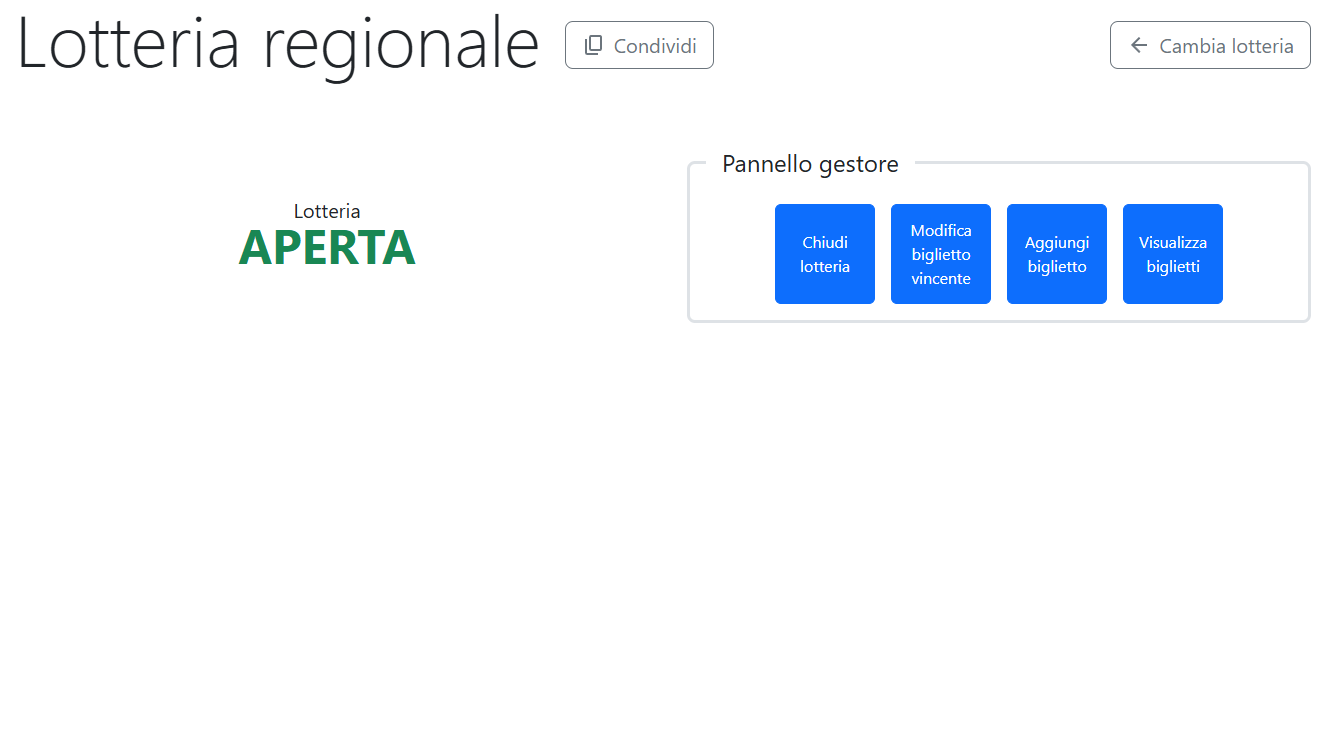
\includegraphics[width=0.97\textwidth]{figures/my_owner_view_open.png}}}

\subfloat[Schermata gestore quando la lotteria è chiusa]{\frame{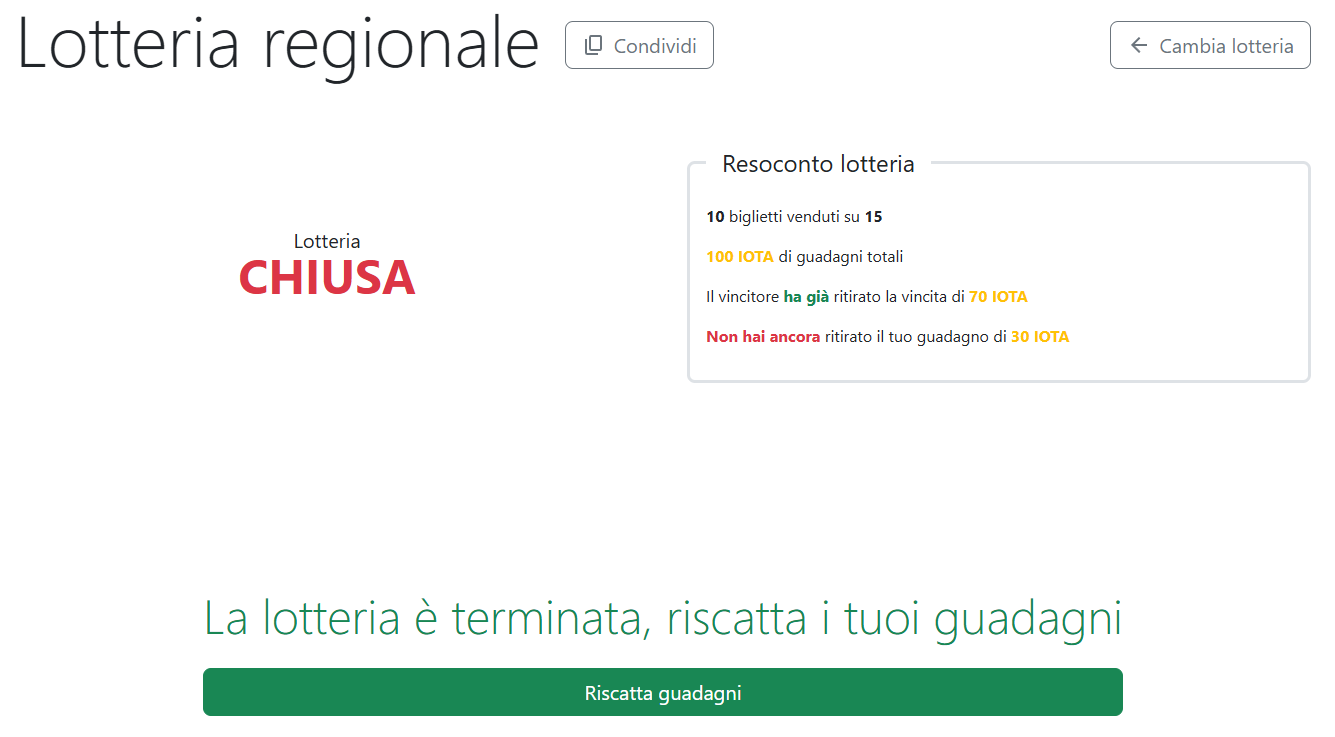
\includegraphics[width=0.97\textwidth]{figures/my_owner_view_closed.png}}}
\caption[Schermata gestore]{Versione finale della schermata gestore}\label{fig:owner_view}
\end{center}
\end{figure}
\pagebreak
\subsubsection{Contenuti di UserView}
Il componente \texttt{UserView.jsx} che mostra la schermata per un partecipante alla lotteria viene caricato in \texttt{Lottery.jsx} quando \texttt{auth} è impostato a \texttt{true} e \texttt{isOwner} a \texttt{false}.\\
\label{app_buy_ticket}Quando la lotteria è aperta, mostra ai partecipanti che ancora non hanno acquistato un biglietto un \texttt{Button} per poter effettuare l'acquisto. Permette quindi di chiamare la funzione \texttt{buy\_ticket} dello smart contract, utilizzando il parametro aggiuntivo \texttt{value: web3.utils.toWei(10, "ether")} per specificare la somma del pagamento (vedi \ref{app_payments}). Se non ci sono biglietti disponibili, verificabile dallo stato \texttt{ticketsAvailable} ottenuto dalla view \texttt{check\_ticket\_availability}, il \texttt{Button} è disattivato. Gli utenti che invece hanno acquistato un biglietto ne visualizzano l'identificativo numerico.\\
Per verificare se l'utente possiede un biglietto e ottenere l'identificativo di tale biglietto in caso positivo, si utilizza un'unica chiamata alla view \texttt{check\_ticket} dello smart contract. Se la chiamata va a buon fine e restituisce il biglietto, lo mostra salvandolo nello stato \texttt{ticket}. Altrimenti, se la chiamata lancia l'errore relativo al mancato possesso del biglietto da parte del chiamante, imposta \texttt{ticket} a \texttt{undefined} che di conseguenza mostra il \texttt{Button} di acquisto. Anche se in questo modo viene permesso il fallimento della transazione, non è impattante in quanto la funzione è una view e quindi non utilizza alcun gas e non richiede nessuna tassa o conferma all'utente.\\
Quando la lotteria è chiusa, se un utente non ha ancora acquistato un biglietto, il \texttt{Button} di acquisto viene disattivato. I partecipanti potranno invece visualizzare un testo che li informa della vincita o perdita, che viene verificato tramite la view \texttt{check\_winner}, il cui risultato viene salvato nello stato \texttt{isWinner}. Al vincitore verrà mostrato anche il \texttt{Button} per incassare la vincita. Tramite lo stato \texttt{isCashedIn} ottenuto dalla view \texttt{cashed\_in}, viene controllato se disattivare il \texttt{Button} quando il vincitore ha già incassato la vincita. Tramite il \texttt{Button} viene quindi chiamata la funzione \texttt{cash\_in\_victory} dello smart contract. Se la vincita viene ritirata con successo, un toast notifica l'utente indicando la quantità di IOTA ricevuti, valore ottenuto chiamando la view \texttt{winning\_amount}.\\
In Figura \ref{fig:user_view} sono riportate le versioni finali della schermata partecipante durante la lotteria aperta e chiusa.

\begin{figure}[H]
\begin{center}
\subfloat[Schermata partecipante quando la lotteria è aperta]{\frame{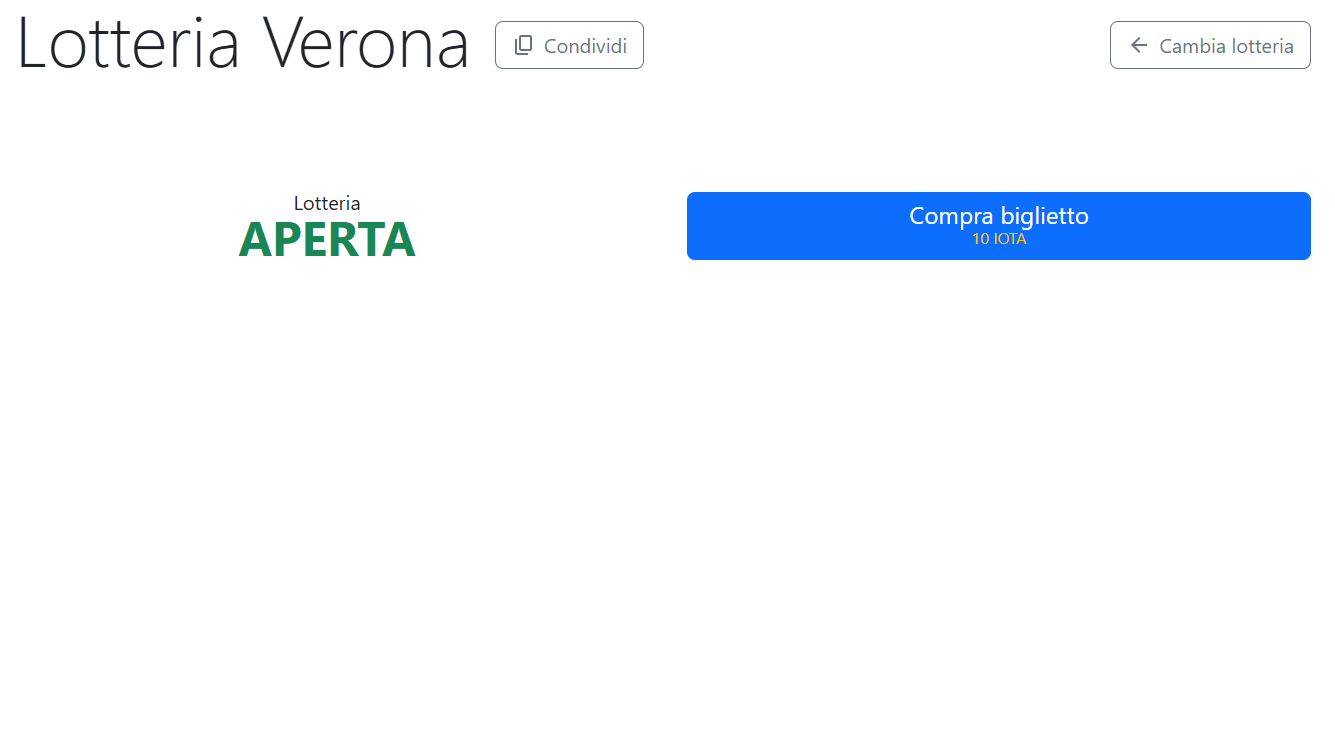
\includegraphics[width=0.97\textwidth]{figures/my_user_view_open.png}}}

\subfloat[Schermata partecipante quando la lotteria è chiusa]{\frame{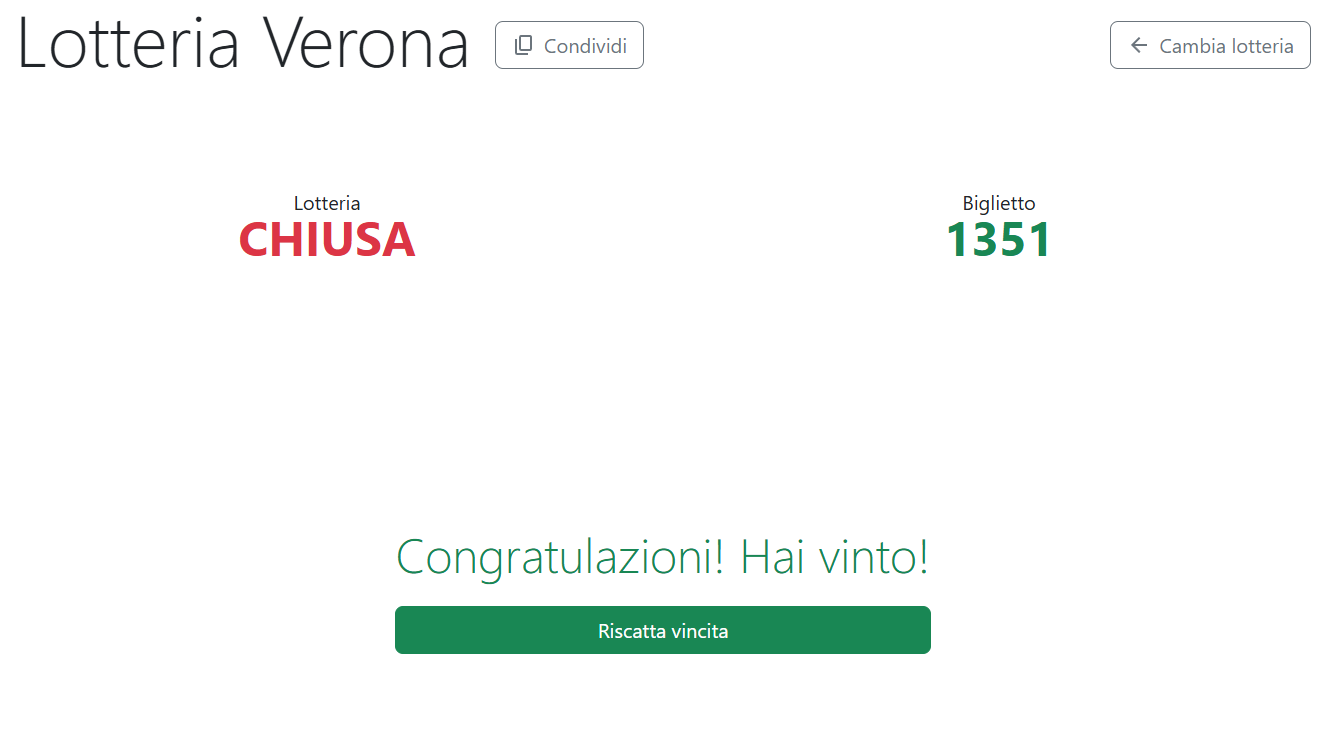
\includegraphics[width=0.97\textwidth]{figures/my_user_view_closed.png}}}
\caption[Schermata partecipante]{Versione finale della schermata partecipante}\label{fig:user_view}
\end{center}
\end{figure}

\subsection{Sviluppo della schermata di accesso}
La seconda fase di sviluppo dell'applicazione web è stata invece dedicata ad implementare la possibilità di creare una lotteria direttamente dall'applicazione, e di accedere a qualsiasi lotteria tramite il suo indirizzo. È stato quindi creato a questo scopo un componente aggiuntivo \texttt{Access.jsx} che viene caricato in \texttt{Lottery.jsx} dopo aver effettuato il collegamento a MetaMask.\\
Per poter creare una lotteria, è stato necessario implementare un metodo per effettuare il deploy di uno smart contract tramite l'applicazione web. Si sono innanzitutto rilevati necessari questi due componenti:
\begin{enumerate}[font=\bfseries]
    \item \textbf{L'\acrshort{abi} dello smart contract}, analogamente ai requisiti per connettersi a uno smart contract già inserito in blockchain (vedi \ref{connect_contract}).
    \item \textbf{Il bytecode del codice dello smart contract}. È possibile ottenerlo dopo aver compilato il codice da Remix. È stato poi successivamente salvato nel file \texttt{bytecode.js} e importato in \texttt{Access.jsx} come costante \texttt{bytecode}.
\end{enumerate}
Nel Codice \ref{lst:app_deploy} è riportato come è stato implementato il deploy di uno smart contract lotteria tramite l'applicazione.
\begin{lstlisting}[language=JSX, caption=Deploy di Smart Contract da applicazione web, label={lst:app_deploy}]
// Utilizzo di ABI e bytecode per generare lo smart contract
const contract = new web3.eth.Contract(abi)
contract.options.data = bytecode
// Creazione della transazione per effettuare il deploy
const gasPrice = await web3.eth.getGasPrice()
const deployedContract = await contract.deploy({arguments: [ticketList, winningTicket, lotteryName]}).send({ from: account, gasPrice: gasPrice })
\end{lstlisting}
Nel codice viene creato un oggetto \texttt{Contract} a partire dall'\acrshort{abi} per gli smart contract lotteria, al quale viene poi fornito il bytecode contenente il codice compilato. Tutto questo viene caricato su blockchain tramite il metodo \texttt{deploy} dell'oggetto. I parametri del costruttore vengono inseriti nel parametro \texttt{arguments} di \texttt{deploy} sotto forma di array. L'oggetto \texttt{deployedContract} ottenuto come risultato della funzione \texttt{deploy} contiene le informazioni dello smart contract appena inserito su blockchain. In particolare, l'indirizzo dello smart contract è reperibile in \texttt{deployedContract.options.address}.\\
Il componente possiede un \texttt{Button} per creare una lotteria, che apre un \texttt{Modal} contenente il form per la creazione. Viene richiesto di inserire un nome per la lotteria di massimo 50 caratteri e di inserire i biglietti uno per volta tramite un input\footnote{Come per l'aggiunta di un biglietto dalla schermata gestore, sono richiesti identificativi univoci da 4 cifre.}. Viene inoltre visualizzata la lista dei biglietti aggiunti fino a quel momento, dalla quale è possibile selezionare quale rendere vincente. All'invio del form, viene effettuato il deploy dello smart contract come visto nel Codice \ref{lst:app_deploy}, utilizzando come parametri per il costruttore i dati inseriti. Successivamente, viene salvato il suo indirizzo in \texttt{contractAddress}, utilizzato poi per creare gli oggetti \texttt{contract} e \texttt{contract\_wss}\footnote{\texttt{contractAddress}, \texttt{contract} e \texttt{contract\_wss}, che prima erano costanti, ora diventano stati React in modo da poter essere modificati.} in modo analogo al procedimento in sezione \ref{connect_metamask}. Una volta creati questi due oggetti, viene caricata la schermata gestore o partecipante.\\
Per poter invece accedere a una lotteria già presente su blockchain, il componente possiede un input nel quale è possibile inserirne l'indirizzo. All'invio, l'indirizzo inserito viene salvato in \texttt{contractAddress}. In questo caso però, prima di poter creare gli oggetti \texttt{Contract} è necessario verificare che l'indirizzo inserito sia valido, e che sia effettivamente l'indirizzo di un'istanza lotteria piuttosto che di un qualsiasi altro smart contract. Viene quindi creato un oggetto \texttt{Contract} temporaneo utilizzato per convalidare l'indirizzo. Per verificare che sia un indirizzo valido, è sufficiente che la creazione dell'oggetto vada a buon fine. In caso di errore, significa che l'indirizzo non è di uno smart contract e quindi è possibile notificare l'utente dell'errore. Per verificare che invece sia un'istanza degli smart contract lotteria, viene effettuato un tentativo di chiamata alla view \texttt{check\_UUID}, utilizzando come parametro una costante \texttt{contract\_UUID} creata nell'applicazione, analoga a quella presente nello smart contract (vedi \ref{uuid}). Se la chiamata fallisce perché la funzione non esiste o perché l'UUID fornito non combacia con quello dello smart contract, l'indirizzo inserito non è di un'istanza lotteria e l'utente viene notificato dell'errore. Altrimenti, l'indirizzo è corretto e vengono creati gli oggetti \texttt{contract} e \texttt{contract\_wss}, caricando la schermata gestore o partecipante.\\
Inoltre, sono stati aggiunti due \texttt{Button} alle schermate gestore e partecipante per integrare adeguatamente la nuova schermata di accesso:
\begin{enumerate}
    \item Un \texttt{Button} per condividere l'indirizzo della lotteria. Permette di copiare nella clipboard l'indirizzo dello smart contract a cui si è connessi, per poter salvare o condividere la lotteria a dei partecipanti.
    \item Un \texttt{Button} per ritornare alla schermata di accesso. Elimina \texttt{contractAddress}, \texttt{contract} e \texttt{contract\_wss}, poiché la mancanza di questi stati causa il caricamento del componente \texttt{Access.jsx}.
\end{enumerate}
In Figura \ref{fig:access_view} è riportata la versione finale della schermata di accesso.

\begin{figure}[h]
\begin{center}
\frame{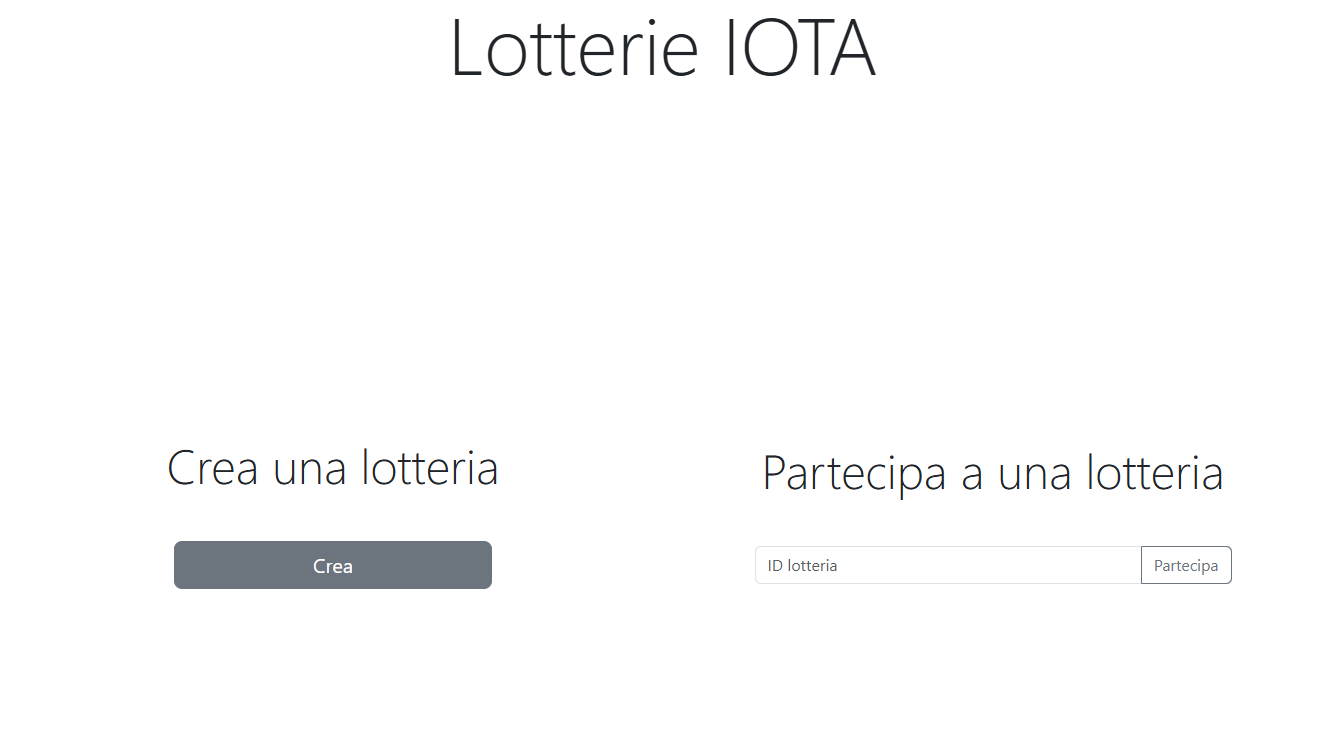
\includegraphics[width=0.98\textwidth]{figures/my_access_view.png}}
\caption[Schermata di accesso]{Schermata di accesso per creare o accedere a una lotteria}\label{fig:access_view}
\end{center}
\end{figure}

\clearpage{\pagestyle{empty}\cleardoublepage}



%%%%%%%%%%%%%%%%%%%%%%%%%%%%%%%%%%%%%%%%
% RISULTATI
\chapter{Risultati}
\label{chap:results}
%Descrivete e inserite qui gli esperimenti effettuati e i dati raccolti. Se avete grafici e dati, presentateli in questa sezione (nella forma in cui pensate sia pi\`u facile visualizzare quello che volete far trasparire dai dati). Scrivete sempre su che supporti hardware o software avete effettuato le prove e quante ne avete fatte (se rilevante).
In questo capitolo viene effettuato un resoconto sui risultati riscontrati dall'utilizzo della programmazione su ledger distribuiti. In particolare, vengono analizzati vantaggi e svantaggi portati dallo sviluppo di applicazioni basate su smart contract rispetto ai classici paradigmi. Viene inoltre analizzata l'efficienza di esecuzione sul ledger scalabile di IOTA, comparandolo anche con quello di Ethereum. 
\section{Vantaggi della programmazione di Smart Contract}
Sono stati riscontrati vari vantaggi dallo sviluppo di un'applicazione su ledger distribuito. Il più rilevante è sicuramente l'alto livello di sicurezza garantito dal ledger, sia per l'autenticazione sia per la gestione degli scambi di denaro, che sono al contempo semplici e veloci da implementare poiché la base per la loro implementazione è già fornita dal ledger. Come infatti descritto nel capitolo precedente, per implementare il sistema di autenticazione è stato sufficiente inserire dei semplici controlli all'interno dello smart contract. I controlli convalidano gli indirizzi degli utenti nel ledger, che sono già autenticati tramite quest'ultimo. In una normale applicazione web, sarebbe invece stato necessario implementare un backend con un sistema di autenticazione molto più complesso, e che non raggiungerebbe comunque lo stesso livello di sicurezza. Lo stesso discorso è valido anche per l'implementazione dei pagamenti: sono infatti sufficienti semplici chiamate di funzione per utilizzare il sistema di pagamenti sicuro e senza autorità centrali del ledger. Per implementare un sistema di pagamento in un'applicazione web che non si basa su ledger distribuiti, sarebbe stato necessario creare un sistema più lungo e complesso\footnote{Sia per l'implementazione che per l'utilizzo finale. I pagamenti sul ledger sono infatti molto rapidi e richiedono pochi passaggi all'utente, rispetto ai sistemi di pagamento tradizionali forniti da autorità terze come banche.}, passando anche per delle autorità terze. Questo risulta spesso anche in tasse sugli acquisti superiori a quelle richieste per utilizzare gas su blockchain.\\
Un altro vantaggio è dato dalla possibilità di utilizzare lo smart contract anche come database dell'applicazione. Tramite i mapping è infatti possibile creare in modo semplice associazioni anche elaborate fra utenti del ledger e strutture dati, tutto salvato in modo sicuro e permanente nello stato della blockchain. Questo evita quindi di implementare un vero e proprio database all'interno di un server dell'applicazione web.\\
Tutti i vantaggi elencati risultano infine nella rimozione della necessità di creare un server backend per l'applicazione web. Tutto è infatti gestito dal ledger stesso, necessitando quindi della sola programmazione di uno smart contract, ma godendo allo stesso tempo di un'elevata sicurezza.\\
Fra gli svantaggi invece, risultano innanzitutto le conseguenze dell'immutabilità degli smart contract. Dopo il deploy non è infatti più in alcun modo possibile modificare lo smart contract, ed è necessaria quindi una grande attenzione prima del deploy per assicurarsi che non saranno necessarie modifiche future. Un altro punto importante è la necessità per gli utenti di possedere account e bilanci all'interno del ledger, cosa che attualmente non è scontata per molti utenti finali. Al momento infatti, i ledger distribuiti sono una tecnologia in crescita e non sono ancora largamente utilizzati. Inoltre, nell'applicazione sono da aspettarsi dei tempi di esecuzione per tutte le operazioni che interagiscono con lo smart contract leggermente più elevati rispetto a quelli su un'applicazione tradizionale. È poi da tenere in considerazione la necessità di pagare tasse per il gas bruciato dalle modifiche allo stato della blockchain, che seppur minimali sono comunque sempre presenti. 

\section{Tempi di esecuzione}
Sono stati inoltre effettuati dei test per valutare l'efficienza di esecuzione dello smart contract.\\
Sono stati innanzitutto testati i tempi di esecuzione delle funzioni view, prendendo come campione la funzione \texttt{is\_lottery\_open}. I dati sono stati raccolti effettuando la chiamata 100 volte, sia sulla testnet IOTA per la quale è stata sviluppata l'applicazione, sia sulla testnet Sepolia di Ethereum. Nella Figura \ref{fig:is_lottery_open_runtime} sono riportati i risultati.

\begin{figure}[h]
\begin{center}
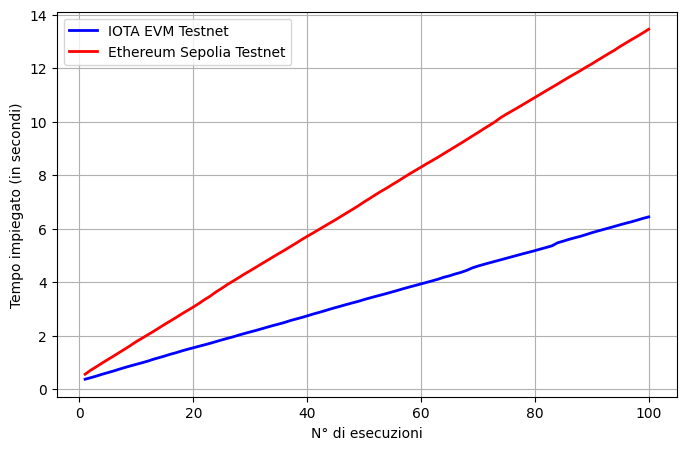
\includegraphics[width=\textwidth]{figures/my_is_lottery_open_runtime.png}
\caption[Tempi di esecuzione view]{Comparazione dei tempi di esecuzione di \texttt{is\_lottery\_open} fra IOTA e Ethereum}\label{fig:is_lottery_open_runtime}
\end{center}
\end{figure}
Da questo grafico si evince che l'efficienza della rete IOTA nell'effettuare operazioni di lettura dello stato è superiore a quella della rete Ethereum. IOTA arriva infatti con 100 esecuzioni ad avere un tempo totale di esecuzione di circa 6 secondi rispetto ai circa 13 secondi di Ethereum, vantando quindi un aumento dell'efficienza di oltre il 100\%.\\
Successivamente sono stati testati i tempi di esecuzione anche delle funzioni di scrittura sullo stato, usando la funzione \texttt{buy\_ticket}\footnote{Per questi test sono stati rimossi alcuni controlli della funzione, in modo da permettere multiple esecuzioni da parte dello stesso indirizzo.} che prevede sia scritture che pagamenti. I risultati sono riportati in Figura \ref{fig:buy_ticket_runtime}.

\begin{figure}[h]
\begin{center}
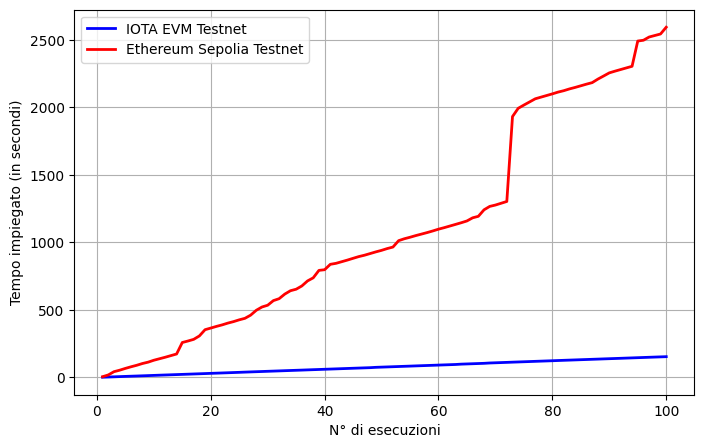
\includegraphics[width=\textwidth]{figures/my_buy_ticket_runtime.png}
\caption[Tempi di esecuzione write]{Comparazione dei tempi di esecuzione di \texttt{buy\_ticket} fra IOTA e Ethereum}\label{fig:buy_ticket_runtime}
\end{center}
\end{figure}
Qui, in un'operazione che prevede pagamenti e modifiche allo stato, è dove la vera efficienza del ledger scalabile di IOTA viene evidenziata. Mentre infatti IOTA mantiene sempre dei tempi ragionevoli, con circa 154 secondi totali dopo 100 esecuzioni, Ethereum invece presenta dei tempi nettamente più elevati. Per effettuare 100 esecuzioni infatti, ha impiegato un tempo totale di circa 2594 secondi, ovvero circa 43 minuti. Una singola esecuzione spaziava da un tempo minimo di 5 secondi fino a un tempo massimo di anche quasi 700 secondi nei momenti in cui la rete era congestionata\footnote{Questi momenti di massimo congestionamento rendono il calcolo delle tempistiche estremamente variabile in base al momento in cui viene svolto il test. Infatti, svolgendo nuovamente il ciclo di 100 esecuzioni in un momento diverso in cui la rete era probabilmente più congestionata, il tempo impiegato ha raggiunto i 7541 secondi, ovvero circa 2 ore.}, con il tempo medio più comune di 10-20 secondi. Grazie all'elevata scalabilità di IOTA e alle sue \acrshort{pow} estremamente leggere per creare una transazione, ogni sua esecuzione ha invece impiegato un tempo costante di circa 1-2 secondi.\\
Infine, sono stati testati anche i tempi di deploy, effettuando un ciclo di esecuzione di 100 deploy sia per IOTA che per Ethereum. I risultati sono riportati in Figura \ref{fig:deploy_runtime}.

\begin{figure}[h]
\begin{center}
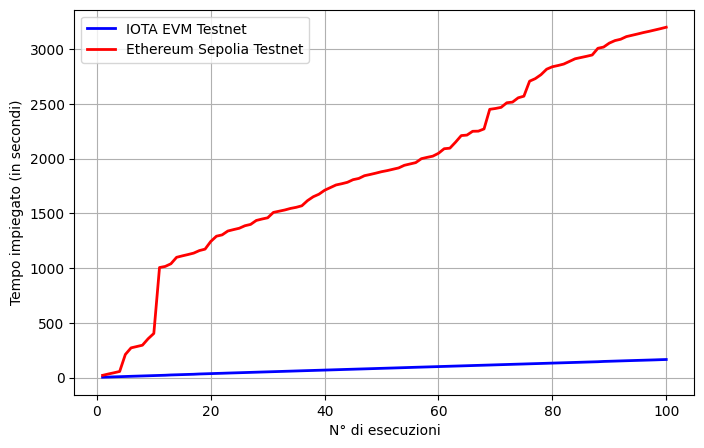
\includegraphics[width=\textwidth]{figures/my_deploy_runtime.png}
\caption[Tempi di esecuzione deploy]{Comparazione dei tempi di esecuzione di un deploy fra IOTA e Ethereum}\label{fig:deploy_runtime}
\end{center}
\end{figure}
Le tempistiche qui sono simili a quelle delle funzioni write, con dei tempi maggiorati per entrambe le reti. Ethereum ha compiuto un tempo totale di circa 3201 secondi, ovvero circa 53 minuti. IOTA invece ha necessitato di un tempo totale di circa 165 secondi. C'è stato quindi un aumento del 23\% per Ethereum rispetto all'esecuzione di una funzione di write, equivalente a 10 minuti in più\footnote{Questi tempi, data l'instabilità delle prestazioni di Ethereum, possono essere molto variabili.}, anche in questo caso con tempistiche estremamente variabili fra singole esecuzioni. IOTA invece, rispetto alla funzione di write ha impiegato soltanto il 6\% di tempo in più, equivalente a 10 secondi, mantenendo inoltre sempre delle tempistiche molto stabili e lineari per ogni singola esecuzione. Questo prova nuovamente l'efficienza e la stabilità del ledger di IOTA rispetto ad altre blockchain come Ethereum.

\clearpage{\pagestyle{empty}\cleardoublepage}



%%%%%%%%%%%%%%%%%%%%%%%%%%%%%%%%%%%%%%%%
% CONCLUSIONI
\chapter{Conclusioni e sviluppi futuri}
\label{chap:conclusion}
%Da scrivere alla fine, un breve riassunto di cosa si \`e affrontato, i risultati (se quanto indicato nell'introduzione come obiettivo \`e stato raggiunto) e come \`e possibile continuare la tesi (p.e. se qualcosa non \`e stato affrontato per motivi di tempo o limitazioni hardware).
In questa tesi sono state analizzate le possibilità e i vantaggi portati dallo sviluppo su piattaforme decentralizzate di ledger distribuiti, facendo luce in particolare su come IOTA Foundation stia portando in questo settore rivoluzioni che puntano a migliorare nettamente efficienza e usabilità delle piattaforme. A tale scopo, sono stati sviluppati uno Smart Contract e un'applicazione esterna che si interfaccia con esso.\\
È stata innanzitutto introdotta la tecnologia di IOTA. Si è visto come la struttura a \acrshort{dag} del Tangle risolva i problemi di scalabilità delle tradizionali strutture di blockchain. Con la successiva integrazione del multi-ledger, IOTA ha poi permesso la creazione di multiple blockchain sopra al Tangle, che agiscono in parallelo potendo anche comunicare fra di loro, su cui possono girare degli smart contract. Vengono analizzati anche i benefici portati dall'aggiornamento IOTA 2.0, che garantisce un'economia bilanciata e sostenibile basata sull'utilizzo di una nuova risorsa chiamata Mana. Inoltre, viene accennato il nuovissimo progetto IOTA Rebased, approvato ufficialmente durante la stesura di questa tesi, che pianifica di unificare in un unico layer il Tangle e la programmazione di smart contract.\\
Successivamente, sono state descritte le specifiche dello smart contract sviluppato e della sua applicazione esterna. Lo smart contract, scritto in Solidity, implementa un sistema di lotterie, permettendo a un'entità di creare e gestire una lotteria. Qualsiasi altra entità può partecipare a una lotteria acquistando un biglietto, e al termine della lotteria sia il vincitore che il gestore possono ritirare una somma di denaro, rispettivamente del 70\% e del 30\% dei guadagni totali ottenuti dalla vendita dei biglietti. L'applicazione esterna permette di interagire con tale smart contract, fornendo la possibilità di creare una lotteria o di partecipare a una già creata, mostrando poi una schermata gestore o partecipante in seguito all'autenticazione dell'utente. A tale scopo viene realizzata un'applicazione web in React e TypeScript, che interagisce con lo smart contract tramite la libreria web3.js e l'estensione web MetaMask.\\
È stato poi illustrato il processo di sviluppo dello smart contract e dell'applicazione web. Lo sviluppo dello smart contract è avvenuto in tre fasi. Durante la prima fase è stata sviluppata la struttura base del sistema di lotteria, implementando le funzionalità progettate. Durante la seconda fase è stato implementato il sistema di pagamenti, che include l'acquisto dei biglietti e il pagamento al gestore e al vincitore alla fine della lotteria. Durante la terza fase invece, sono stati implementati eventi e view aggiuntive per permettere all'applicazione di interfacciarsi correttamente con lo smart contract. Lo sviluppo dello smart contract si è rivelato semplice e senza particolari problemi o limitazioni. Lo sviluppo dell'applicazione web è invece avvenuto implementando inizialmente le schermate gestore e partecipante, e utilizzando un unico smart contract hardcoded nell'applicazione. Successivamente, è stata implementata anche la schermata che permette di creare uno smart contract lotteria direttamente dall'applicazione e di connettersi a uno già creato. Durante lo sviluppo dell'applicazione web sono stati riscontrati alcuni problemi, principalmente legati alla gestione degli eventi emessi dallo smart contract. È stato infatti rilevato che, quando un evento viene ricevuto dall'applicazione, lo smart contract potrebbe non aver ancora salvato le modifiche effettuate allo stato dalla funzione che ha emesso l'evento. Quindi, quando l'applicazione necessitava del nuovo stato dello smart contract per gestire l'evento, è stato necessario inserire dei tempi di attesa per permettere allo smart contract di aggiornarsi.\\
Infine, sono stati analizzati i principali vantaggi e svantaggi riscontrati durante lo sviluppo di un'applicazione su piattaforme di ledger distribuiti. Lo sviluppo si è rivelato particolarmente vantaggioso per quanto riguarda l'elevata sicurezza e la semplicità nell'implementarla. L'autenticazione, lo scambio di denaro, e il salvataggio di dati in un database sono infatti gestiti dal ledger e facilmente implementabili nello smart contract, rendendo sufficiente lo sviluppo di un'applicazione frontend che si interfacci con esso senza necessitare di un server backend. Inoltre, grazie alla natura del ledger, gli scambi di denaro sono sicuri, veloci, e non necessitano di autorità centrali. Le complessità da tenere in considerazione invece, includono la necessità di prestare particolare attenzione alla correttezza del codice prima di effettuare il deploy di uno smart contract, in quanto successivamente non può più essere modificato in alcun modo. Inoltre, la necessità per gli utenti di possedere un account sul ledger potrebbe influire negativamente sulla distribuzione dell'applicativo. Attualmente infatti, questo è un settore recente e ancora in fase di sviluppo e crescita, con un'utenza più ristretta rispetto ai possibili utilizzatori di un'applicazione sviluppata in modo tradizionale. Si presenta anche la necessità per gli utenti di pagare tasse in gas per l'utilizzo dell'applicazione, e di attendere tempi maggiori per il completamento delle operazioni. È stato analizzato anche quanto il ledger di IOTA fornisca prestazioni più elevate rispetto ad altri sistemi tradizionali di blockchain. I risultati ottenuti riportano infatti tempi dimezzati per effettuare operazioni di lettura, e tempi enormemente inferiori per effettuare operazioni di scrittura. Questo dimostra quanto sia reale il bottleneck dato dalla struttura tradizionale di blockchain, e quanto invece sia positivamente impattante la struttura scalabile a \acrshort{dag} di IOTA.\\
Per portare avanti il lavoro svolto durante questa tesi, è possibile continuare ad approfondire un sistema per implementare in modo più efficiente la gestione degli eventi. Un'implementazione da tenere in considerazione potrebbe partire dall'idea di effettuare periodicamente i controlli dopo la ricezione dell'evento\footnote{Ad esempio, ogni 3 secondi per 15 secondi, invece che una sola volta dopo 10 secondi.} per rendere più reattiva la risposta, nonostante però questo implichi multiple transazioni aggiuntive da dover effettuare. Inoltre, è da tenere in considerazione che durante lo sviluppo del progetto è stato annunciato che la libreria utilizzata web3.js verrà archiviata\footnote{\url{https://blog.chainsafe.io/web3-js-sunset/}}, con l'avvio del processo a marzo 2025. La libreria creata da Ethereum Foundation è stata la prima storica libreria per comunicare con smart contract. Nel 2020 fu ceduta a ChainSafe per proseguirne la manutenzione e lo sviluppo\footnote{\href{https://medium.com/chainsafe-systems/chainsafe-receives-grant-from-ef-for-web3js-9e4376f5f36a}{\texttt{https://medium.com/chainsafe-systems/chainsafe-receives-grant-from-ef-for -web3js-9e4376f5f36a}}}, e in definitiva è stato deciso a gennaio 2025 di terminarne il supporto per promuovere la crescita di altre librerie più recenti. Quindi, un passo importante per proseguire il lavoro di tesi deve essere quello di considerare l'implementazione con una nuova libreria, come ethers.js o Viem, che sono attualmente le più promettenti fra le librerie in crescita riguardanti la comunicazione con reti di blockchain.\\
In generale, il lavoro svolto in questa tesi propone un esempio di come i programmi sviluppati su ledger distribuiti possano essere utilizzati in contesti reali, e punta a mostrare quanto sia vantaggioso scegliere di supportare e utilizzare le tecnologie proposte da IOTA Foundation. Pertanto, questo lavoro è ampiamente proseguibile anche continuando a sviluppare smart contract su IOTA e ad analizzare possibili casi di utilizzo a cui questi possono essere applicati, implementando magari anche sistemi di tokenizzazione avanzata spiegati in sezione \ref{utxo_extension}, e approcciandosi allo sviluppo sul nuovo IOTA Rebased con il più avanzato linguaggio Move della MoveVM.\

\clearpage{\pagestyle{empty}\cleardoublepage}



%%%%%%%%%%%%%%%%%%%%%%%%%%%%%%%%%%%%%%%%%%
% RIMUOVERE LE APPENDICI SE NON UTILIZZATE
%imposta l'intestazione di pagina
\renewcommand{\chaptermark}[1]{\markright{\thechapter \ #1}{}}
\lhead[\fancyplain{}{\bfseries\thepage}]{\fancyplain{}{\bfseries\rightmark}}
\appendix %imposta le appendici
\chapter{Compilazione e deploy tramite Remix} %crea l'appendice
\label{chap:deploy}
%In questa Appendice non si \`e utilizzato il comando:\\
%\verb"" è equivalente all' ambiente verbatim,  ma si utilizza all'interno di un discorso.
%\verb"\clearpage{\pagestyle{empty}\cleardoublepage}", ed infatti l'ultima pagina 8 ha l'intestazione con il numero di pagina in alto.

In questa appendice sono riportati i passi da seguire per poter effettuare il deploy di uno smart contract su blockchain, tramite l'IDE di Remix.
\begin{enumerate}
    \item Accedere all'IDE, disponibile al seguente link: \url{https://remix.ethereum.org/}.
    \item Inserire il file con il codice dello smart contract nel file explorer online di Remix, oppure caricarlo dal proprio filesystem locale tramite il plugin \textit{remixd}\footnote{\url{https://remix-ide.readthedocs.io/en/latest/remixd.html}}.
    \item Compilare il codice:
    \begin{enumerate}
        \item Accedere alla sezione \textbf{Solidity Compiler} di Remix e avviare la compilazione.
        \item Come risultato, è inoltre possibile copiare l'\acrshort{abi} e il bytecode dello smart contract.
    \end{enumerate}
    \pagebreak
    \item \label{enum:provider}Connettersi a un provider. Per questo progetto, è stato utilizzato MetaMask\footnote{\url{https://metamask.io/}}:
    \begin{enumerate}
        \item Creare un wallet con uno o più account.
        \item Collegarsi alla rete del ledger tramite il provider. Per questo progetto, è stata utilizzata la testnet di IOTA, i cui dati per la connessione sono forniti al seguente link: \url{https://wiki.iota.org/build/networks-endpoints/#iota-evm-testnet}.
    \end{enumerate}
    \item \label{enum:faucet}Ottenere dei token nell'account desiderato. Nel caso della testnet, è possibile ottenere fondi gratuitamente tramite faucet al seguente link: \url{https://evm-toolkit.evm.testnet.iotaledger.net/}.
    \item Effettuare il deploy:
    \begin{enumerate}
        \item Accedere alla sezione \textbf{Deploy \& run transactions} di Remix.
        \item Selezionare come \textbf{ENVIRONMENT} il provider ottenuto nel passo \ref{enum:provider}.
        \item Selezionare l'account tramite il quale si vuole effettuare il deploy.
        \item Inserire i parametri di input del costruttore e avviare \textbf{Deploy}.
    \end{enumerate}
    \item Lo smart contract sarà poi stato inserito su blockchain e sarà possibile monitorarlo e interagirci tramite Remix nella sezione \textbf{Deployed Contracts}.
\end{enumerate}

%imposta l'intestazione di pagina
\rhead[\fancyplain{}{\bfseries \thechapter \:Prima Appendice}]
{\fancyplain{}{\bfseries\thepage}}



\clearpage{\pagestyle{empty}\cleardoublepage}



\chapter{Utilizzare l'applicazione web}
In questa appendice sono riportati i passi da seguire per poter avviare ed utilizzare l'applicazione web.
\begin{enumerate}
    \item Installare MetaMask come provider e connettersi alla testnet IOTA, seguendo il passo \ref{enum:provider} dell'Appendice \ref{chap:deploy}.
    \item Ottenere fondi sulla testnet seguendo il passo \ref{enum:faucet} dell'Appendice \ref{chap:deploy}.
    \item Installare Node.js e npm\footnote{\url{https://docs.npmjs.com/downloading-and-installing-node-js-and-npm}}.
    \item Avviare un terminale all'interno della cartella di progetto.
    \item Eseguire il comando \texttt{npm install} e attendere l'installazione dei moduli dell'applicazione.
    \item Eseguire \texttt{npm run start} e attendere l'avvio automatico dell'applicazione web sul browser.
\end{enumerate}

\rhead[\fancyplain{}{\bfseries \thechapter \:Seconda Appendice}]
{\fancyplain{}{\bfseries\thepage}}


\clearpage{\pagestyle{empty}\cleardoublepage}
%%%%%%%%%%%%%%%%%%%%%%%%%%%%%%%%%%%%%%%%%
% BIBLIOGRAFIA
\addcontentsline{toc}{chapter}{Bibliografia}
\label{Bibliography}
\bibliographystyle{IEEEtran}
\bibliography{src/bibliography}
\rhead[\fancyplain{}{\bfseries Bibliografia}]
{\fancyplain{}{\bfseries\thepage}}
\end{document}